% This is the Reed College LaTeX thesis template. Most of the work
% for the document class was done by Sam Noble (SN), as well as this
% template. Later comments etc. by Ben Salzberg (BTS). Additional
% restructuring and APA support by Jess Youngberg (JY).
% Your comments and suggestions are more than welcome; please email
% them to cus@reed.edu
%
% See https://www.reed.edu/cis/help/LaTeX/index.html for help. There are a
% great bunch of help pages there, with notes on
% getting started, bibtex, etc. Go there and read it if you're not
% already familiar with LaTeX.
%
% Any line that starts with a percent symbol is a comment.
% They won't show up in the document, and are useful for notes
% to yourself and explaining commands.
% Commenting also removes a line from the document;
% very handy for troubleshooting problems. -BTS

% As far as I know, this follows the requirements laid out in
% the 2002-2003 Senior Handbook. Ask a librarian to check the
% document before binding. -SN

%%
%% Preamble
%%
% \documentclass{<something>} must begin each LaTeX document
\documentclass[12pt,oneside]{reedthesis}
% Packages are extensions to the basic LaTeX functions. Whatever you
% want to typeset, there is probably a package out there for it.
% Chemistry (chemtex), screenplays, you name it.
% Check out CTAN to see: https://www.ctan.org/
%%
\usepackage{graphicx,latexsym}
%\usepackage{amsmath}
\usepackage{amssymb,amsthm}
\usepackage{longtable,booktabs,setspace}
\usepackage{chemarr} %% Useful for one reaction arrow, useless if you're not a chem major
\usepackage[hyphens]{url}
% Added by CII
\usepackage{hyperref}
\usepackage{lmodern}
\usepackage{float}
\floatplacement{figure}{H}
% Thanks, @Xyv
\usepackage{calc}
% End of CII addition
\usepackage{rotating}

% Next line commented out by CII
%%% \usepackage{natbib}
% Comment out the natbib line above and uncomment the following two lines to use the new
% biblatex-chicago style, for Chicago A. Also make some changes at the end where the
% bibliography is included.
%\usepackage{biblatex-chicago}
%\bibliography{thesis}

\renewcommand{\tablename}{Tabla}

% Added by CII (Thanks, Hadley!)
% Use ref for internal links
\renewcommand{\hyperref}[2][???]{\autoref{#1}}
\def\chapterautorefname{Capítulo}
\def\sectionautorefname{Sección}
\def\subsectionautorefname{Subsección}
% End of CII addition

% Added by CII
\usepackage{caption}
\captionsetup{width=5in}
% End of CII addition

% \usepackage{times} % other fonts are available like times, bookman, charter, palatino

% Syntax highlighting #22

% To pass between YAML and LaTeX the dollar signs are added by CII
\title{Caracterización morfológica, fisiológica y molecular de entradas de algodón (\emph{Gossypium hirsutum} L.) e identificación de QTL de importancia agronómica}
\author{Ing. Agr. Pablo Nahuel Dileo}
% The month and year that you submit your FINAL draft TO THE LIBRARY (May or December)
\date{Versión 1.5}
\division{Facultad de Ciencias Agrarias}
\advisor{Dr.~Gustavo Rubén Rodríguez}
\institution{Universidad Nacional del Nordeste}
\degree{Doctorado en Recursos Naturales}
%If you have two advisors for some reason, you can use the following
% Uncommented out by CII
\altadvisor{Dr.~Marcelo Javier Paytas}
% End of CII addition

%%% Remember to use the correct department!
\department{Doctorado}
% if you're writing a thesis in an interdisciplinary major,
% uncomment the line below and change the text as appropriate.
% check the Senior Handbook if unsure.
%\thedivisionof{The Established Interdisciplinary Committee for}
% if you want the approval page to say "Approved for the Committee",
% uncomment the next line
%\approvedforthe{Committee}

% Added by CII
%%% Copied from knitr
%% maxwidth is the original width if it's less than linewidth
%% otherwise use linewidth (to make sure the graphics do not exceed the margin)
\makeatletter
\def\maxwidth{ %
  \ifdim\Gin@nat@width>\linewidth
    \linewidth
  \else
    \Gin@nat@width
  \fi
}
\makeatother

% From {rticles}

\renewcommand{\contentsname}{Tabla de Contenidos}
% End of CII addition

\setlength{\parskip}{0pt}

% Added by CII

\providecommand{\tightlist}{%
  \setlength{\itemsep}{0pt}\setlength{\parskip}{0pt}}

\Acknowledgements{
Agradecimientos aquí..
}

\Dedication{
Dedicatoria aquí..
}

\Publications{
Lista de publicaciones a congresos y revistas aquí..
}

\Resumen{
Primer párrafo del resumen en español.

\par

Segundo párrafo del resumen aquí.
}

\Abstract{
Primer párrafo del resumen en inglés.

\par

Segundo párrafo del resumen aquí.
}

    \usepackage{graphicx}
    \usepackage{latexsym}
    \usepackage{fontspec}
    \setmainfont[Ligatures=TeX]{Calibri}
    \usepackage{amsmath}
    \usepackage[spanish]{babel}
    \addto\captionsspanish{\renewcommand{\tablename}{Tabla}}
    \addto\captionsspanish{\renewcommand{\chaptername}{Capítulo}}
    \addto\captionsspanish{\renewcommand{\listtablename}{Índice de Tablas}}
    \addto\captionsspanish{\renewcommand{\listfigurename}{Índice de Figuras}}
    \addto\captionsspanish{\renewcommand{\contentsname}{Índice General}}
    \usepackage{setspace}
    \onehalfspacing
    \usepackage{geometry}
    \geometry{a4paper,left=3cm,right=3cm,top=2.5cm,bottom=2.5cm}
    \usepackage[style=apa, backend=biber]{biblatex}
    \addbibresource{referencias.bib}
    \usepackage{hyperref}
    \usepackage{csquotes}
    \usepackage{booktabs}
    \usepackage{longtable}
    \usepackage{array}
    \usepackage{multirow}
    \usepackage{wrapfig}
    \usepackage{float}
    \usepackage{colortbl}
    \usepackage{pdflscape}
    \usepackage{tabu}
    \usepackage{threeparttable}
    \usepackage{threeparttablex}
    \usepackage[normalem]{ulem}
    \usepackage{makecell}
    \usepackage{xcolor}
% End of CII addition
%%
%% End Preamble
%%
%
% Personalización de encabezado y pie de página 
\usepackage{fancyhdr} 
\pagestyle{fancy} 
\fancyhf{} % Limpia todos los encabezados y pies de página
\fancyhead{} % Limpia cualquier encabezado preexistente
\fancyfoot[R]{\thepage} % Coloca el número de página en la parte inferior derecha
\renewcommand{\headrulewidth}{0pt} % Eliminar línea en el encabezado 
\renewcommand{\footrulewidth}{0pt} % Eliminar línea en el pie de página


% Paquete necesario para configurar el espacio entre títulos
\usepackage{titlesec}  

% Configuración de interlineado general
\setstretch{1.5}  % Interlineado general de 1.5

% Configuración del espacio entre títulos y texto
\titlespacing*{\chapter}{0pt}{20pt}{10pt}  % Ajusta el espacio antes y después de los títulos de capítulos
\titlespacing*{\section}{0pt}{15pt}{5pt}   % Ajusta el espacio antes y después de los títulos de secciones
\titlespacing*{\subsection}{0pt}{10pt}{5pt} % Ajusta el espacio antes y después de los títulos de subsecciones

% Espacio entre párrafos
\setlength{\parskip}{1.5ex plus 0.5ex minus 0.5ex}  % Aumenta el espacio entre párrafos


\begin{document}

% Paginación en números romanos para las secciones preliminares
\frontmatter 
\pagestyle{empty} % this removes page numbers from the frontmatter
\pagenumbering{roman} 
\fancyfoot[R]{\thepage}

  \maketitle

  \begin{acknowledgements}
    Agradecimientos aquí..
    \thispagestyle{fancy} % Asegura que se utiliza el estilo de paginación fancy para esta página 
    \fancyhf{} % Limpia encabezados y pies de página 
    \fancyhead{} % Limpia cualquier encabezado preexistente 
    \fancyfoot[R]{\thepage} % Coloca el número de página en la parte inferior derecha
    %\setcounter{page}{3} % Establece el contador de página en 1
  \end{acknowledgements}

  \begin{dedication}
    Dedicatoria aquí..
    \thispagestyle{fancy} % Asegura que se utiliza el estilo de paginación fancy para esta página 
    \fancyhf{} % Limpia encabezados y pies de página 
    \fancyhead{} % Limpia cualquier encabezado preexistente 
    \fancyfoot[R]{\thepage} % Coloca el número de página en la parte inferior derecha
  \end{dedication}

  \begin{publications}
    Lista de publicaciones a congresos y revistas aquí..
    \thispagestyle{fancy} % Asegura que se utiliza el estilo de paginación fancy para esta página 
    \fancyhf{} % Limpia encabezados y pies de página 
    \fancyhead{} % Limpia cualquier encabezado preexistente 
    \fancyfoot[R]{\thepage} % Coloca el número de página en la parte inferior derecha
  \end{publications}

  \hypersetup{linkcolor=black}
  \setcounter{secnumdepth}{2}
  \setcounter{tocdepth}{2}
  \tableofcontents
  \thispagestyle{fancy} % Asegura que se utiliza el estilo de paginación fancy para esta página 
    \fancyhf{} % Limpia encabezados y pies de página 
    \fancyhead{} % Limpia cualquier encabezado preexistente 
    \fancyfoot[R]{\thepage} % Coloca el número de página en la parte inferior derecha

\chapter*{Lista de Abreviaturas}
\begin{table}[h]
    \centering
    \begin{tabular}{ll}
                \textbf{A1RR} & Altura a primer rama reproductiva \\
                \textbf{AP} & Altura de planta \\
                \textbf{D1P} & Distancia de la primera posición al tallo principal \\
                \textbf{IF} & Índice de fibra \\
                \textbf{IS} & Índice de semillas \\
                \textbf{IU} & Índice de uniformidad de fibras \\
                \textbf{Mic} & Micronaire \\
                \textbf{N1RR} & Nudos a primer rama reproductiva \\
                \textbf{NC} & Número de capullos \\
                \textbf{NN} & Número de nudos \\
                \textbf{NRR} & Número de ramas reproductivas \\
                \textbf{NRV} & Número de ramas vegetativas \\
                \textbf{NSC} & Numero de semillas por capullo \\
                \textbf{PC} & Peso promedio de capullos \\
                \textbf{RB} & Rendimiento de algodón bruto \\
                \textbf{RF} & Rendimiento de fibra \\
                \textbf{RFD} & Rendimiento de fibra al desmote \\
                \textbf{Str} & Resistencia de las fibras \\
                \textbf{UHML} & Longitud de las fibras \\
                \textbf{zContinua...} & Otras abreviaturas \\
            \end{tabular}
\end{table}
\thispagestyle{fancy} % Asegura que se utiliza el estilo de paginación fancy para esta página 
    \fancyhf{} % Limpia encabezados y pies de página 
    \fancyhead{} % Limpia cualquier encabezado preexistente 
    \fancyfoot[R]{\thepage} % Coloca el número de página en la parte inferior derecha

  \begin{resumen}
    Primer párrafo del resumen en español.

    \par

    Segundo párrafo del resumen aquí.
    \thispagestyle{fancy} % Asegura que se utiliza el estilo de paginación fancy para esta página 
    \fancyhf{} % Limpia encabezados y pies de página 
    \fancyhead{} % Limpia cualquier encabezado preexistente 
    \fancyfoot[R]{\thepage} % Coloca el número de página en la parte inferior derecha
  \end{resumen}

  \begin{abstract}
    Primer párrafo del resumen en inglés.

    \par

    Segundo párrafo del resumen aquí.
    \thispagestyle{fancy} % Asegura que se utiliza el estilo de paginación fancy para esta página 
    \fancyhf{} % Limpia encabezados y pies de página 
    \fancyhead{} % Limpia cualquier encabezado preexistente 
    \fancyfoot[R]{\thepage} % Coloca el número de página en la parte inferior derecha
  \end{abstract}

  \listoftables
  \thispagestyle{fancy} % Asegura que se utiliza el estilo de paginación fancy para esta página 
  \fancyhf{} % Limpia encabezados y pies de página 
  \fancyhead{} % Limpia cualquier encabezado preexistente 
  \fancyfoot[R]{\thepage} % Coloca el número de página en la parte inferior derecha

  \listoffigures
  \thispagestyle{fancy} % Asegura que se utiliza el estilo de paginación fancy para esta página 
  \fancyhf{} % Limpia encabezados y pies de página 
  \fancyfoot[R]{\thepage} % Coloca el número de página en la parte inferior derecha
  \renewcommand{\headrulewidth}{0pt} % Elimina la línea en el encabezado para esta sección

% Configuración de encabezados y pies de página
\pagestyle{fancy}  % Activa el estilo fancyhdr para los encabezados y pies de página
\fancyhf{}  % Limpia los encabezados y pies de página predeterminados


% Eliminar mayúsculas en los encabezados
\renewcommand{\chaptermark}[1]{\markboth{\thechapter\ #1}{}}
\renewcommand{\sectionmark}[1]{\markright{\thesection\ #1}}

% Configuración del encabezado
\fancyhead[L]{\fontsize{10}{12}\selectfont \leftmark}  % Título del capítulo a la izquierda con tamaño 10
\fancyhead[C]{\fontsize{10}{12}\selectfont}            % (Opcional) El centro puede estar vacío con tamaño 10
\fancyhead[R]{\fontsize{10}{12}\selectfont \rightmark} % Título de la sección a la derecha con tamaño 10

% Configuración del pie de página
\fancyfoot[C]{}           % (Opcional) El centro del pie de página puede estar vacío
\fancyfoot[L]{}           % (Opcional) El pie de página izquierdo puede estar vacío
\fancyfoot[R]{\thepage}   % Número de página a la derecha en el pie de página
\fancyfoot[R]{\fontsize{10}{12}\selectfont \thepage} % Coloca el número de página en la parte inferior derecha con tamaño 10

\mainmatter % here the regular arabic numbering starts
\pagestyle{fancyplain} % turns page numbering back on
\renewcommand{\headrulewidth}{0.4pt} % Agregar línea en el encabezado


\chapter*{Introducción}\label{introducciuxf3n}
\addcontentsline{toc}{chapter}{Introducción}

El algodón (\emph{Gossypium hirsutum} L.) se cultiva en más de 80 países y desempeña un papel crucial en la producción textil como fuente de fibra. Argentina es el segundo productor de algodón de América Latina después de Brasil y desempeña un papel clave en los sistemas productivos de la región noreste del país. La producción de fibra cubre la demanda interna a la vez que facilita la exportación a países como Vietnam, Pakistán, Turquía, China, Indonesia, Colombia e India \autocite{icac2023,paytas2013}. Se han desarrollado nuevas variedades y sistemas de producción para adaptarse a diversas condiciones medioambientales. En Argentina, el Instituto Nacional de Tecnología Agropecuaria (INTA) cuenta con un programa de mejora genética del algodón que utiliza el germoplasma disponible para desarrollar variedades que mejoren el rendimiento y la calidad de la fibra. El programa ha logrado aumentar tanto el rendimiento como la calidad de la fibra y también ha incorporado la resistencia genética a enfermedades importantes como mancha angular, enfermedad azul y marchitez por fusarium, en numerosas variedades \autocite{royo2007,scarpin2022,scarpin2023}.

Recientemente, \textcite{scarpin2022} informaron de un progreso genético en el rendimiento de fibra, el porcentaje de desmote, el rendimiento de algodón bruto y el número de cápsulas (NC), mostrando una tasa media de crecimiento anual de 3,24 kg ha\textsuperscript{-1}, 0,05 \%, 4,86 kg ha\textsuperscript{-1} y 0,12 NC, respectivamente. Como resultado, las variedades más modernas tienen un mayor rendimiento de fibra, porcentaje de desmote, rendimiento de algodón bruto y número de cápsulas que las variedades más antiguas. Estos resultados indican que los programas de mejoramiento genético del algodón en Argentina han logrado un progreso genético sustancial para el rendimiento de fibra y sus componentes. Además, \textcite{scarpin2023} enfatizaron que este progreso no resultó en una disminución de la calidad del algodón. Sin embargo, se necesita más investigación para mejorar el rendimiento de fibra, la calidad de la fibra y la adaptabilidad a diferentes ambientes. En la provincia de Santa Fe (Argentina), el cultivo de algodón se concentra en los departamentos de 9 de Julio, Vera y General Obligado, cada uno de los cuales presenta disparidades distintivas en cuanto a la composición del suelo y las condiciones ambientales. El tipo de clima en el norte de la provincia es subtropical según la clasificación climática de Köppen, con una estación seca en la región noroeste y sin estación seca en la región noreste de la provincia \autocite{anida2024}. Debido a estas diferencias, es esencial desarrollar genotipos para estas diferentes condiciones para avanzar en la mejora de los cultivos. Además, se necesitan esfuerzos adicionales para identificar genes o QTLs asociados con rasgos agronómicos y de calidad de fibra en variedades de algodón en Argentina a través de métodos de mapeo genético.

En un programa de mejora genética del algodón, combinar un alto rendimiento y calidad de la fibra es un reto clave. El primer paso crucial para un programa de mejora eficaz es caracterizar el germoplasma del algodón. \textcite{kearsey1996} destacaron la importancia de comprender las diferencias genéticas y la heredabilidad de los rasgos al momento de cruzar plantas. La heredabilidad muestra en qué medida los rasgos están influidos por la genética y puede estimarse comparando las varianzas de las generaciones segregantes y no segregantes. En el algodón, se han notificado estimaciones de heredabilidad para varios rasgos, como el rendimiento de fibra, los componentes del rendimiento, la calidad de la fibra, la altura de la planta, el aceite de semilla, el nudo de la primera rama reproductiva, la cápsulas a prueba de tormentas, entre otros \autocite{meredith1984,tang1996,ribeiro2017,decarvalho2022,nidagundi2023}. Estos estimadores ayudan a los mejoradores a decidir la

selección individual y a predecir cuánto pueden mejorar ciertos rasgos. Sin embargo, merece la pena tener en cuenta que el nivel de heredabilidad cambia en función del rasgo, la población y el ambiente en el que se cultivan.



















































\chapter{\texorpdfstring{Caracterización de entradas de algodón (\emph{Gossypium hirsutum} L.) del banco de germoplasma de INTA mediante caracteres morfo-fisiológicos}{Caracterización de entradas de algodón (Gossypium hirsutum L.) del banco de germoplasma de INTA mediante caracteres morfo-fisiológicos}}\label{rmd-basics}

\section{Introducción}\label{introducciuxf3n-1}

Aquí una breve introducción del capítulo\\

\section{Objetivos}\label{objetivos}

Caracterizar entradas de algodón del banco de germoplasma de INTA con diferente procedencia mediante caracteres morfológicos relacionados al rendimiento.

Evaluar procesos fisiológicos que intervienen en la determinación del rendimiento de fibra de entradas de algodón del banco de germoplasma de INTA.

\section{Materiales y métodos}\label{materiales-y-muxe9todos}

Los ensayos se realizaron en invernadero con condiciones controladas en la Estación Experimental INTA Reconquista. Se utilizaron macetas de 5 litros con 2,2 Kg de suelo de monte (pH: 6,7, P disp: 165,7 mg Kg\textsuperscript{-1}, Na\textsuperscript{+} 0,6 cmol\textsuperscript{+}Kg\textsuperscript{-1}, K\textsuperscript{+}: 0,8 cmol\textsuperscript{+}Kg\textsuperscript{-1}, Ca\textsuperscript{+2}: 27,0 cmol\textsuperscript{+}Kg\textsuperscript{-1}, Mg\textsuperscript{+2}: 2,2 cmol\textsuperscript{+}Kg\textsuperscript{-1}, NH\textsubscript{4}: 76,30 mg kg\textsuperscript{-1}, NO\textsubscript{3}: 86,1 mg Kg\textsuperscript{-1}) y de 400 g de sustrato comercial (GrowMix Multipro), en el cual se colocó una planta por maceta.

\subsection{\texorpdfstring{Caracterización morfológica de 26 entradas de algodón (\emph{Gossypium hirsutum} L.)}{Caracterización morfológica de 26 entradas de algodón (Gossypium hirsutum L.)}}\label{caracterizaciuxf3n-morfoluxf3gica-de-26-entradas-de-algoduxf3n-gossypium-hirsutum-l.}

En el estudio se llevó a cabo una caracterización inicial de 26 entradas (Tabla \ref{tab:tablaEntradas}) de algodón (\emph{Gossypium hirsutum} L.) del banco de germoplasma utilizando un diseño experimental en bloques completos al azar con tres repeticiones.

\begin{table}[!h]
\centering
\caption{\label{tab:tablaEntradas}Entradas de \emph{Gossypium hirsutum} L. y su procedencia}
\centering
\resizebox{\ifdim\width>\linewidth\linewidth\else\width\fi}{!}{
\begin{threeparttable}
\begin{tabular}[t]{>{\raggedright\arraybackslash}p{8em}>{\raggedright\arraybackslash}p{12em}ll}
\toprule
Entradas  & Procedencia  & Entradas & Procedencia\\
\midrule
BGSP-00166* & Argentina & BGSP-00748 & China\\
BGSP-00177 & Argentina & BGSP-00752 & China\\
BGSP-00192 & Argentina & BGSP-00755 & China\\
BGSP-00193 & Argentina & BGSP-00759 & China\\
BGSP-00194 & Argentina & BGSP-00779 & China\\
\addlinespace
BGSP-00207* & Argentina & BGSP-00067 & Costa de Marfil\\
BGSP-00269* & Argentina & BGSP-00028 & EEUU\\
SP 41255* & Argentina-Línea avanzada & BGSP-00145 & EEUU\\
SP 6565* & Argentina-Línea avanzada & BGSP-00159* & EEUU\\
BGSP-00514 & Australia & BGSP-00425* & EEUU\\
\addlinespace
BGSP-00072 & Camerún & BGSP-00428 & EEUU\\
BGSP-00088 & Camerún & BGSP-00715 & Pakistán\\
BGSP-00070 & Chad & BGSP-00126* & Senegal\\
\bottomrule
\end{tabular}
\begin{tablenotes}[para]
\item \textit{Referencias:} 
\item * Entradas que fueron seleccionadas para un mayor análisis
\end{tablenotes}
\end{threeparttable}}
\end{table}

\subsubsection{Variables medidas}\label{variables-medidas}

Las variables que se mencionan a continuación fueron registradas en todas las plantas de las 26 entradas:

\begin{enumerate}
\def\labelenumi{\roman{enumi})}
\item
  Características morfológicas cualitativas: Estas variables se registraron durante la etapa de floración de las plantas según los descriptores de INASE \texttt{(colocar\ cita)}. Forma de la planta, aspecto de la canopia, tipo de floraciones, forma y pubescencia de la hoja, tipo de bráctea y forma de cápsula.
\item
  Características morfológicas cuantitativas: Las mediciones se realizaron en la etapa de final de ciclo de las plantas, siguiendo estos métodos: Altura de planta (AP en cm, medido desde la base del tallo hasta el ápice), Altura a la primera rama reproductiva (A1RR en cm, medido desde la base del tallo hasta la primera rama reproductiva), número de nudos (NN, número de nudos presentes en el tallo), número de ramas vegetativas (NRV) y reproductivas (NRR), nudo de inserción de la primera rama reproductiva (N1RR, nudo donde se inserta la 1º rama reproductiva en la planta), y distancia de la primera posición al tallo principal (D1P en cm, distancia que existe entre el tallo principal y la primera posición de la primera rama reproductiva de la planta).
\item
  Rendimiento y sus componentes: Para calcular el rendimiento de las diferentes entradas y sus componentes se efectuaron las siguientes mediciones: Rendimiento bruto de algodón (RB, en g): se recolectó la fibra-semilla de algodón de todas las cápsulas presentes en las plantas. Las muestras obtenidas fueron pesadas en balanzas de precisión y se realizó medición de la humedad de cada una de ellas; Rendimiento de fibra al desmote (RFD, en \%): se tomó cada muestra de algodón proveniente de las mediciones de rendimiento bruto, se realizó el desmote en una mini-desmotadora experimental y se pesó en una balanza de precisión la fibra y semillas por separado. El rendimiento de fibra al desmote fue la relación entre el peso de la fibra sobre el peso de la fibra más la semilla; Rendimiento de fibra (RF en g): se multiplicó el rendimiento bruto de algodón por el rendimiento de fibra al desmote obtenido; Nº de cápsulas por planta (NC): se determinó mediante recuento de todas las cápsulas presentes en las plantas; Peso de cápsulas (PC): se dividió el rendimiento bruto de algodón por planta por el número de cápsula por plantas
\item
  Parámetros de calidad tecnológica de fibra de algodón: con el total de plantas de cada entrada se hizo un pool de muestras para obtener una medición debido a los requisitos de peso mínimo de muestra de fibra del instrumento de medición. Las muestras de fibra de algodón obtenidas se enviaron al laboratorio de HVI (Uster 1000) de la Asociación para la Promoción de la Producción (APPA) en Reconquista, Santa Fe. Los parámetros de calidad tecnológica de fibra registrados fueron: Índice de Hilabilidad (SCI, por sus siglas en inglés), Micronaire (Mic), Índice de madurez (Mac), longitud promedio de la mitad superior (UHML en mm, por sus siglas en inglés), longitud media (ML, por sus siglas en inglés), índice de uniformidad (UI en \%, por sus siglas en inglés), índice de fibras cortas (SFI, por sus siglas en inglés), resistencia de fibra (Str en g tex\textsuperscript{-1}), elongación (Elg en \%), contenido de humedad de la muestra, color (Rd y +b), grado de color (C.G) y contenido de basura.
\item
  Fenología: Tiempo en días desde la emergencia para alcanzar los estados de primer pimpollo (DPP), primera flor abierta (DPF), cut out (DCO), primera bocha abierta (DPCA) y fin de ciclo (DFC). El estado de cut out o fin de floración efectiva se determina cuando el número de nudos por encima de la última flor blanca en el tallo sea menor que 4 \autocite{bourland1992}.
\end{enumerate}

\subsection{\texorpdfstring{Caracterización de ocho entradas seleccionadas de algodón (\emph{Gossypium hirsutum} L.)}{Caracterización de ocho entradas seleccionadas de algodón (Gossypium hirsutum L.)}}\label{caracterizaciuxf3n-de-ocho-entradas-seleccionadas-de-algoduxf3n-gossypium-hirsutum-l.}

Las ocho entradas fueron seleccionadas por sus características contrastantes en rendimiento, sus componentes (principalmente RFD) y calidad de fibra. También se incluyeron algunas con bajo número de RV y canopia compacta. Estas entradas, identificadas con un asterisco en la Tabla \ref{tab:tablaEntradas}, también fueron evaluadas para analizar procesos fisiológicos involucrados en la determinación del rendimiento de fibra en algodón.

\subsubsection{Variables medidas}\label{variables-medidas-1}

La medición de las variables fisiológicas, como fotosíntesis, contenido de clorofila y apertura y cierre estomático, se llevaron a cabo en tres momentos durante el ciclo de la planta, correspondiente a 55, 70 y 85 días después de la emergencia. Fue realizado en un solo año de evaluación con un diseño experimental en bloques completos al azar. Los equipos utilizados para las mediciones propuestas fueron a) Fotosíntesis: LICOR 6400; b) Contenido de clorofila: Minolta SPAD 502; c) Apertura y cierre estomático: LICOR 6400.

Para profundizar el análisis, se realizaron experimentos adicionales repetidos en dos momentos, con nueve repeticiones cada vez, utilizando un diseño en bloques completos al azar. Se aumentó la cantidad de bloques para mejorar la representatividad de los parámetros de calidad de fibra y permitir un análisis estadístico más preciso. Se registraron las variables de rendimiento y calidad de fibra mencinados anteriormente sumado las siguientes variables: número de semillas por cápsula (NSC)\autocite{worley1974}, índice de fibra (IF en g, peso de la fibra proveniente de 100 semillas) y el índice de semillas (IS en g, peso de 100 semillas de cada muestra) \autocite{pettigrew2013}.

Por otra parte, se realizaron muestreos destructivos de plantas para la determinación de materia seca y partición de los asimilados. Los cortes se realizaron a los 30, 60, 90 y 120 días (correspondientes a los estados fenológicos 1er pimpollo, 1era flor, 1era bocha abierta y fin de ciclo). En cada uno de estos momentos se seccionaron las plantas en tallo, ramas reproductivas, ramas vegetativas, pimpollos y flores, bochas cerradas, capsulas abiertas, fibra y rebrote de tallo según el momento de muestreo. Todas las muestras de las partes de la planta fueron llevadas a estufa a 65 º C hasta peso constante (96 horas). El ensayo se realizó en un diseño en bloques al azar con arreglo en parcelas divididas, con los 4 momentos de corte y las entradas incluidas en cada parcela, con cuatro repeticiones. En estos cuatros momentos mencionados tambien se midieron las siguientes variables: Área foliar: para el cálculo de esta variable, se midieron todas las hojas de las plantas a través de los equipos LICOR 3000 y LICOR 3050; viii) Dinámica de la floración: se realizaron mapeos de dinámica de floración en todas las plantas seleccionadas para la partición de asimilados. Este procedimiento se realiza registrando en cada una de las posiciones reproductivas que genera la planta, la presencia de un pimpollo, una flor, una bocha verde, una cápsula abierta o un aborto \autocite{kerby1996monitoring}. Con estos datos se realizó la dinámica de floración de las diferentes entradas y porcentaje de retención final a la que llegan cada una de las plantas seleccionadas para el mapeo.

\subsection{Análisis estadístico}\label{anuxe1lisis-estaduxedstico}

Análisis estadístico de 26 entradas

\texttt{Falta\ detallar\ analisis}

Análisis estadístico de ocho entradas

Para la caracterización de la ocho entradas de algodón, se realizaron análisis de varianza (ANOVA) y análisis de correlación de Pearson de todos los rasgos medidos utilizando el software R \autocite{R2024}. La distribución normal de cada rasgo se confirmó mediante la prueba de Shapiro-Wilk. Las diferencias estadísticas se evaluaron con un nivel de confianza del 95 \% (p ≤ 0,05) según la prueba L.S.D de Fisher, considerando las entradas como efecto fijo, mientras que el experimento y los bloques dentro de cada experimento como efectos aleatorios. Luego, se realizó un estudio completo de la diversidad genética disponible en ese conjunto de entradas mediante el análisis de componentes principales.

\section{Resultados}\label{resultados}

\subsection{\texorpdfstring{Caracterización morfológica de 26 entradas de algodón (\emph{Gossypium hirsutum} L.)}{Caracterización morfológica de 26 entradas de algodón (Gossypium hirsutum L.)}}\label{caracterizaciuxf3n-morfoluxf3gica-de-26-entradas-de-algoduxf3n-gossypium-hirsutum-l.-1}

\subsubsection{Características morfológicas cualitativas}\label{caracteruxedsticas-morfoluxf3gicas-cualitativas}

La tabla \ref{tab:tabla-descriptores} detalla las características de las entradas del banco de germoplasma de algodón evaluadas. En términos de la forma de la planta, el 61,5\% fueron cilíndricas y el 38,5\% fueron cónicas. En cuanto al aspecto de la canopia, se destacaron las categorías ``medio'' (69,2\%) y ``abierta'' (23,1\%). Sin embargo, algunas antradas presentaron una canopia ``compacta'' (7,7\%), como los genotipos BGSP-00166 y BGSP-00194. El tipo de floración varió entre individual (23,1\%), agrupada (7,7\%) o medio agrupada (69,2\%). Las hojas se presentan principalmente en forma palmada (96,1\%) y plana (96,1\%), y el resto en forma digitada (3,9\%) y en copa (3,9\%) , con niveles variados de pubescencia (11,5\% para pubescencia escasa y fuerte, y 76,9\% para pubescencia media). Solo la entrada BGSP-00514 presentó forma digitada o también conocida como tipo ``Okra''. En todas las entradas, el tipo de bráctea es normal, mientras que la forma de la bocha varió entre cónica (88,5\%), elíptica (7,7\%) y redonda (3,8\%).

\begin{table}[!h]
\centering\centering
\caption{\label{tab:tabla-descriptores}Descriptores}
\centering
\resizebox{\ifdim\width>\linewidth\linewidth\else\width\fi}{!}{
\fontsize{12}{14}\selectfont
\begin{tabular}[t]{lllllllll}
\toprule
\multicolumn{1}{c}{ } & \multicolumn{3}{c}{Característica de planta} & \multicolumn{3}{c}{Característica de hoja} & \multicolumn{1}{c}{Bráctea} & \multicolumn{1}{c}{Cápsula} \\
\cmidrule(l{3pt}r{3pt}){2-4} \cmidrule(l{3pt}r{3pt}){5-7} \cmidrule(l{3pt}r{3pt}){8-8} \cmidrule(l{3pt}r{3pt}){9-9}
\begingroup\fontsize{12}{14}\selectfont \textbf{Entradas}\endgroup & \begingroup\fontsize{12}{14}\selectfont \textbf{Forma}\endgroup & \begingroup\fontsize{12}{14}\selectfont \textbf{Canopia}\endgroup & \begingroup\fontsize{12}{14}\selectfont \textbf{Tipo Floración}\endgroup & \begingroup\fontsize{12}{14}\selectfont \textbf{Forma  }\endgroup & \begingroup\fontsize{12}{14}\selectfont \textbf{Lámina}\endgroup & \begingroup\fontsize{12}{14}\selectfont \textbf{Pubescencia}\endgroup & \begingroup\fontsize{12}{14}\selectfont \textbf{Tipo}\endgroup & \begingroup\fontsize{12}{14}\selectfont \textbf{Forma }\endgroup\\
\midrule
BGSP-00028 & Cónica & Abierta & Individual & Palmada & Plana & Escasa & Normal & Cónica\\
BGSP-00067 & Cónica & Abierta & Individual & Palmada & Plana & Escasa & Normal & Cónica\\
BGSP-00070 & Cilíndrica & Medio & Medio Agrupada & Palmada & Plana & Media & Normal & Cónica\\
BGSP-00072 & Cilíndrica & Medio & Medio Agrupada & Palmada & Plana & Media & Normal & Cónica\\
BGSP-00088 & Cónica & Medio & Individual & Palmada & Plana & Fuerte & Normal & Cónica\\
\addlinespace
BGSP-00126 & Cilíndrica & Medio & Medio Agrupada & Palmada & Plana & Escasa & Normal & Cónica\\
BGSP-00145 & Cónica & Medio & Individual & Palmada & Plana & Media & Normal & Cónica\\
BGSP-00159 & Cilíndrica & Medio & Medio Agrupada & Palmada & Plana & Media & Normal & Cónica\\
BGSP-00166 & Cilíndrica & Compacta & Agrupada & Palmada & Plana & Media & Normal & Cónica\\
BGSP-00177 & Cónica & Abierta & Medio Agrupada & Palmada & Plana & Media & Normal & Cónica\\
\addlinespace
BGSP-00192 & Cilíndrica & Medio & Medio Agrupada & Palmada & Plana & Media & Normal & Cónica\\
BGSP-00193 & Cilíndrica & Medio & Medio Agrupada & Palmada & Plana & Media & Normal & Cónica\\
BGSP-00194 & Cilíndrica & Compacta & Agrupada & Palmada & Plana & Media & Normal & Cónica\\
BGSP-00207 & Cónica & Abierta & Individual & Palmada & Plana & Fuerte & Normal & Cónica\\
BGSP-00269 & Cilíndrica & Medio & Medio Agrupada & Palmada & Plana & Media & Normal & Cónica\\
\addlinespace
BGSP-00425 & Cilíndrica & Medio & Medio Agrupada & Palmada & Plana & Media & Normal & Cónica\\
BGSP-00428 & Cilíndrica & Medio & Medio Agrupada & Palmada & Plana & Media & Normal & Redonda\\
BGSP-00514 & Cónica & Abierta & Individual & Digitada (Okra) & Plana & Media & Normal & Cónica\\
BGSP-00715 & Cónica & Medio & Medio Agrupada & Palmada & Plana & Fuerte & Normal & Cónica\\
BGSP-00748 & Cónica & Medio & Medio Agrupada & Palmada & Plana & Media & Normal & Elíptica\\
\addlinespace
BGSP-00752 & Cónica & Medio & Medio Agrupada & Palmada & Plana & Media & Normal & Cónica\\
BGSP-00755 & Cilíndrica & Medio & Medio Agrupadas & Palmada & Plana & Media & Normal & Cónica\\
BGSP-00759 & Cilíndrica & Abierta & Medio Agrupada & Palmada & En copa & Media & Normal & Redonda\\
BGSP-00779 & Cilíndrica & Medio & Medio Agrupada & Palmada & Plana & Media & Normal & Cónica\\
SP 41255 & Cilíndrica & Medio & Medio Agrupada & Palmada & Plana & Media & Normal & Cónica\\
\addlinespace
SP 6565 & Cilíndrica & Medio & Medio Agrupada & Palmada & Plana & Media & Normal & Cónica\\
\bottomrule
\end{tabular}}
\end{table}

\subsubsection{Características morfológicas cuantitativas, rendimiento y sus componentes y calidad de fibra}\label{caracteruxedsticas-morfoluxf3gicas-cuantitativas-rendimiento-y-sus-componentes-y-calidad-de-fibra}

La tabla \ref{tab:tabla-datos-conjuntos} muestra los valores medios de las características morfológicas evaluadas de las entradas del banco de germoplasma de algodón (\emph{Gossypium hirsutum} L.), incluyendo la altura de planta (AP), número de nudos (NN), número de ramas vegetativas (NRV), número de ramas reproductivas (NRR), nudos a la primera rama reproductiva (N1RR), altura a la primera rama reproductiva (A1RR) y distancia de la primera posición al tallo principal (D1P). Los valores de estos parámetros variaron significativamente entre las entradas, con alturas de planta que oscilaron entre 89,0 cm y 126,3 cm, y números de nudos entre 13,0 y 17,0. El número de ramas vegetativas fluctuaron entre 0,3 y 2,7, mientras que el número de ramas reproductivas varió entre 9,7 y 13,3. Los nudos a la primera rama reproductiva estuvieron entre 3,7 a 5,7, y la altura a la primera rama reproductiva varió de 25,0 cm a 40,7 cm. La distancia de la primera posición al tallo principal osciló entre 3,9 cm y 14,3 cm.

La tabla \ref{tab:tabla-datos-conjuntos} también presenta un resumen de las características de rendimiento, calidad de fibra y fenología de las entradas. Los parámetros medidos incluyen rendimiento bruto de algodón (RB), rendimiento de fibra (RF), rendimiento de fibra al desmote (RFD), peso promedio de capullos (PC), número de capullos (NC), longitud promedio de fibra de la mitad superior (UHML), resistencia de las fibras (Str), micronaire (Mic), índice de uniformidad de fibras (IU), días a primer pimpollo (DPP), días a primera flor (DPF), días a cut out (DCO), días a primera cápsula abierta (DPCA) y días a fin de ciclo (DFC). Los valores muestran una amplia variabilidad entre las entradas, con rendimientos brutos de algodón que oscilaron entre 14,3 g planta\textsuperscript{-1} y 33,5 g planta\textsuperscript{-1}, rendimientos de fibra que varió de 4,6 g planta\textsuperscript{-1} a 12,3 g planta\textsuperscript{-1}, peso promedio de capullo entre 2,6 g a 4,7 g y número de capullos entre 4,7 a 8,7. La calidad de la fibra se refleja en características como UHML, que varió de 25,1 mm a 33,9 mm, y la resistencia de las fibras, que osciló entre 21,5 g tex\textsuperscript{-1} y 37,6 g tex\textsuperscript{-1}. En términos fenológicos, los días a primer pimpollo varió de 22 a 27 días, los días a primera flor de 49 a 55 días, los días a cut out de 73 a 80 días, los días a primera cápsula abierta de 113 a 137 días, y los días a fin de ciclo de 161 a 164 días.

\begin{landscape}\begin{table}[!h]
\centering
\caption{\label{tab:tabla-datos-conjuntos}Datos conjuntos...}
\centering
\resizebox{\ifdim\width>\linewidth\linewidth\else\width\fi}{!}{
\begin{threeparttable}
\begin{tabular}[t]{>{\raggedright\arraybackslash}p{6em}lllllllllllllllllllll}
\toprule
\multicolumn{1}{c}{ } & \multicolumn{7}{c}{Características morfológicas} & \multicolumn{5}{c}{Rendimiento y sus componentes} & \multicolumn{4}{c}{Calidad de fibra} & \multicolumn{5}{c}{Fenología} \\
\cmidrule(l{3pt}r{3pt}){2-8} \cmidrule(l{3pt}r{3pt}){9-13} \cmidrule(l{3pt}r{3pt}){14-17} \cmidrule(l{3pt}r{3pt}){18-22}
Entradas & AP & NN & NRV & NRR & N1RR & A1RR & D1P & RB & RF & RFD & PC & NC & UHML & Str & Mic & IU & DPP & DPF & DCO & DPCA & DFC\\
\midrule
 &  &  &  &  &  &  &  &  &  &  &  &  &  &  &  &  &  &  &  &  \vphantom{1} & \\
BGSP-00028 & 106,3 (5,5) & 13,3 (0,9) & 1,0 (0,6) & 10,7 (0,7) & 3,7 (0,3) & 25,3 (0,7) & 9,3 (0,7) & 24,1 (2,0) & 8,7 (0,6) & 36,5 (0,7) & 4,3 (0,3) & 5,7 (0,3) & 30,7 & 34,0 & 3,1 & 84,1 & 25 & 51 & 74 & 118 & 163\\
BGSP-00067 & 102,0 (4,0) & 14,7 (0,7) & 1,3 (0,3) & 11,0 (0,6) & 4,7 (0,3) & 27,0 (1,7) & 11,0 (1,5) & 23,3 (3,3) & 8,2 (1,0) & 36,0 (1,9) & 2,8 (0,2) & 8,3 (1,2) & 26,8 & 37,0 & 2,9 & 80,8 & 25 & 54 & 74 & 128 & 163\\
BGSP-00070 & 109,3 (0,3) & 14,3 (0,3) & 1,3 (0,3) & 9,7 (0,3) & 5,7 (0,7) & 40,7 (4,2) & 9,7 (1,9) & 19,9 (1,3) & 7,7 (0,8) & 39,6 (0,8) & 3,4 (0,3) & 6,0 (0,6) & 32,5 & 31,0 & 3,8 & 84,6 & 27 & 53 & 76 & 128 & 163\\
BGSP-00072 & 113,3 (4,3) & 17,0 (0,0) & 1,3 (0,3) & 13,3 (0,3) & 4,7 (0,3) & 27,3 (3,2) & 7,3 (1,8) & 26,3 (2,2) & 9,8 (0,9) & 38,3 (0,6) & 3,5 (0,4) & 7,7 (0,3) & 28,1 & 28,2 & 4,3 & 82,6 & 25 & 54 & 80 & 130 & 162\\
\addlinespace
BGSP-00088 & 104,3 (5,8) & 14,3 (0,7) & 1,7 (0,3) & 10,7 (0,3) & 4,7 (0,3) & 28,3 (2,7) & 14,3 (1,2) & 31,0 (3,2) & 11,3 (1,1) & 37,1 (0,4) & 4,4 (0,2) & 7,0 (0,6) & 31,6 & 36,5 & 3,5 & 86,2 & 25 & 54 & 78 & 135 & 163\\
BGSP-00126 & 126,3 (3,8) & 14,9 (0,2) & 1,5 (0,2) & 11,3 (0,3) & 4,6 (0,1) & 37,4 (1,4) & 8,9 (0,9) & 16,0 (0,6) & 6,6 (0,3) & 42,9 (0,3) & 2,7 (0,2) & 6,0 (0,3) & 29,9 & 32,4 & 2,8 & 83,5 & 25 & 54 & 79 & 132 & 163\\
BGSP-00145 & 89,0 (4,5) & 14,3 (0,3) & 1,0 (0,6) & 11,3 (0,3) & 4,0 (0,0) & 25,7 (0,9) & 9,7 (1,8) & 16,1 (3,1) & 6,1 (1,1) & 38,6 (0,7) & 3,6 (0,6) & 4,7 (0,9) & 26,9 & 26,6 & 3,5 & 80,8 & 25 & 52 & 73 & 121 & 163\\
BGSP-00159 & 104,3 (3,6) & 14,3 (0,3) & 1,1 (0,2) & 11,0 (0,2) & 4,3 (0,2) & 31,8 (1,9) & 11,4 (0,6) & 14,3 (0,6) & 5,1 (0,2) & 36,8 (0,6) & 2,7 (0,1) & 5,2 (0,2) & 30,0 & 34,4 & 2,5 & 82,7 & 22 & 49 & 74 & 114 & 161\\
BGSP-00166 & 109,0 (3,0) & 15,2 (0,2) & 0,8 (0,2) & 11,8 (0,3) & 4,4 (0,2) & 30,6 (1,2) & 3,9 (0,6) & 18,2 (0,5) & 5,5 (0,2) & 31,1 (0,4) & 3,6 (0,1) & 5,1 (0,2) & 33,9 & 37,6 & 2,5 & 86,1 & 23 & 52 & 74 & 124 & 163\\
\addlinespace
BGSP-00177 & 103,7 (3,3) & 14,3 (0,3) & 1,7 (0,3) & 10,7 (0,3) & 4,7 (0,3) & 32,7 (3,4) & 13,7 (1,7) & 24,5 (2,2) & 7,9 (0,8) & 33,0 (0,4) & 4,2 (0,8) & 6,0 (0,6) & 29,2 & 30,7 & 4,2 & 82,9 & 26 & 53 & 75 & 127 & 164\\
BGSP-00192 & 101,3 (5,8) & 15,0 (0,0) & 1,7 (0,3) & 11,0 (0,0) & 5,0 (0,0) & 29,0 (2,1) & 11,3 (0,9) & 18,7 (3,3) & 7,1 (1,1) & 37,9 (2,0) & 3,3 (0,4) & 5,7 (0,3) & 28,2 & 31,9 & 3,5 & 83,3 & 25 & 54 & 76 & 124 & 162\\
BGSP-00193 & 106,7 (5,5) & 15,3 (0,3) & 2,7 (0,3) & 11,3 (0,3) & 5,0 (0,0) & 30,7 (0,9) & 8,0 (1,7) & 29,4 (3,9) & 10,9 (1,4) & 38,1 (1,8) & 4,2 (0,6) & 7,0 (0,0) & 30,2 & 33,8 & 3,5 & 85,5 & 25 & 55 & 78 & 137 & 162\\
BGSP-00194 & 92,7 (3,2) & 14,7 (0,3) & 2,3 (0,3) & 10,7 (0,3) & 5,0 (0,0) & 31,3 (0,7) & 5,7 (3,2) & 24,0 (3,1) & 9,6 (1,4) & 40,9 (0,8) & 3,7 (0,4) & 6,7 (0,9) & 29,9 & 32,6 & 3,7 & 85,0 & 25 & 55 & 75 & 118 & 163\\
BGSP-00207 & 105,0 (8,5) & 15,3 (0,2) & 0,7 (0,2) & 12,2 (0,2) & 4,2 (0,1) & 29,4 (0,8) & 10,1 (1,0) & 16,2 (0,6) & 6,7 (0,2) & 43,6 (0,5) & 2,8 (0,1) & 5,8 (0,2) & 28,6 & 28,4 & 2,8 & 83,2 & 23 & 52 & 79 & 135 & 164\\
\addlinespace
BGSP-00269 & 113,0 (3,7) & 14,7 (0,2) & 1,2 (0,2) & 11,2 (0,2) & 4,4 (0,1) & 34,2 (1,6) & 8,3 (0,8) & 16,9 (0,5) & 7,1 (0,3) & 43,7 (0,5) & 2,9 (0,2) & 6,1 (0,3) & 29,2 & 33,4 & 3,9 & 84,1 & 23 & 52 & 75 & 133 & 163\\
BGSP-00425 & 105,2 (3,3) & 13,8 (0,1) & 0,9 (0,3) & 10,8 (0,1) & 4,0 (0,0) & 25,5 (0,7) & 8,4 (0,9) & 15,1 (0,5) & 4,6 (0,2) & 31,5 (0,3) & 2,6 (0,1) & 5,8 (0,3) & 32,1 & 32,6 & 2,3 & 82,2 & 25 & 53 & 73 & 130 & 163\\
BGSP-00428 & 105,3 (7,3) & 15,3 (0,3) & 0,7 (0,3) & 12,0 (0,6) & 4,3 (0,3) & 28,0 (2,9) & 8,7 (2,4) & 21,4 (3,6) & 8,7 (1,4) & 40,1 (0,4) & 4,3 (0,7) & 5,0 (0,6) & 25,1 & 23,1 & 4,0 & 80,0 & 23 & 49 & 74 & 113 & 163\\
BGSP-00514 & 99,0 (8,0) & 16,0 (0,0) & 2,7 (0,3) & 12,3 (0,3) & 4,7 (0,3) & 25,0 (1,5) & 11,7 (1,7) & 28,0 (2,8) & 11,7 (1,2) & 42,3 (0,4) & 4,2 (0,2) & 6,7 (0,9) & 29,0 & 32,0 & 2,7 & 83,6 & 23 & 52 & 76 & 117 & 161\\
BGSP-00715 & 102,0 (8,5) & 14,7 (0,9) & 0,3 (0,3) & 11,7 (0,9) & 4,0 (0,0) & 27,3 (2,3) & 13,0 (1,2) & 24,0 (3,6) & 9,8 (1,2) & 41,6 (1,2) & 3,4 (0,4) & 7,0 (0,6) & 27,2 & 31,7 & 4,0 & 83,5 & 24 & 55 & 78 & 134 & 163\\
\addlinespace
BGSP-00748 & 105,7 (0,9) & 15,0 (0,0) & 1,7 (0,3) & 12,0 (0,0) & 4,0 (0,0) & 25,7 (1,2) & 12,0 (0,6) & 33,5 (1,8) & 12,3 (1,0) & 39,0 (2,4) & 4,4 (0,1) & 7,7 (0,3) & 26,3 & 21,5 & 3,9 & 80,9 & 23 & 52 & 74 & 135 & 164\\
BGSP-00752 & 103,3 (5,2) & 15,3 (0,3) & 2,7 (0,3) & 11,3 (0,3) & 5,0 (0,0) & 29,3 (0,7) & 10,3 (0,9) & 27,2 (2,1) & 11,3 (1,2) & 42,1 (1,9) & 4,1 (0,1) & 6,7 (0,3) & 31,8 & 26,7 & 3,6 & 84,1 & 25 & 55 & 79 & 135 & 162\\
BGSP-00755 & 97,3 (3,3) & 13,0 (0,0) & 2,7 (0,3) & 10,0 (0,0) & 4,0 (0,0) & 28,7 (0,3) & 10,3 (0,7) & 26,3 (2,0) & 10,0 (0,7) & 38,5 (0,8) & 4,7 (0,2) & 5,7 (0,7) & 29,8 & 31,4 & 3,3 & 84,2 & 25 & 53 & 75 & 124 & 163\\
BGSP-00759 & 108,3 (5,0) & 14,0 (0,6) & 1,0 (0,6) & 10,0 (1,0) & 5,0 (0,6) & 38,3 (5,5) & 9,7 (2,4) & 24,6 (3,6) & 8,7 (1,5) & 38,3 (1,1) & 4,7 (0,6) & 5,7 (1,5) & 27,8 & 23,9 & 4,1 & 82,3 & 25 & 54 & 77 & 134 & 163\\
BGSP-00779 & 112,3 (1,9) & 16,0 (0,0) & 1,3 (0,3) & 12,3 (0,3) & 4,7 (0,3) & 30,3 (1,8) & 11,7 (0,7) & 26,3 (1,5) & 10,4 (0,5) & 40,5 (0,7) & 3,0 (0,1) & 8,7 (0,3) & 30,2 & 31,5 & 2,7 & 84,4 & 25 & 55 & 76 & 126 & 161\\
\addlinespace
SP 41255 & 122,3 (2,9) & 15,2 (0,1) & 1,2 (0,2) & 11,8 (0,2) & 4,4 (0,1) & 32,7 (1,1) & 11,2 (0,8) & 20,7 (0,7) & 8,8 (0,4) & 44,7 (0,5) & 2,8 (0,1) & 7,3 (0,3) & 30,9 & 32,3 & 3,0 & 84,1 & 23 & 52 & 76 & 124 & 162\\
SP 6565 & 120,8 (1,9) & 15,7 (0,2) & 1,3 (0,2) & 12,2 (0,2) & 4,5 (0,2) & 35,8 (1,6) & 8,4 (0,6) & 17,3 (0,5) & 6,9 (0,2) & 41,2 (0,3) & 2,6 (0,1) & 6,8 (0,3) & 29,9 & 33,3 & 3,0 & 84,6 & 25 & 55 & 79 & 131 & 162\\
 &  &  &  &  &  &  &  &  &  &  &  &  &  &  &  &  &  &  &  &  & \\
p-valor & <0,001 & <0,001 & <0,001 & <0,001 & <0,001 & <0,001 & <0,001 & <0,001 & <0,001 & <0,001 & <0,001 & <0,001 & - & - & - & - & - & - & - & - & -\\
L.S.D Fisher & 17,96 & 1 & 0,99 & 1,05 & 0,74 & 6,29 & 3,89 & 4,3 & 1,76 & 2,46 & 0,76 & 1,42 & - & - & - & - & - & - & - & - & -\\
\bottomrule
\end{tabular}
\begin{tablenotes}[para]
\item \textit{Referencias:} 
\item AP: Altura de planta en cm; NN: Número de nudos; NRV: Número de ramas vegetativas; NRR: Número de ramas reproductivas; N1RR: Nudos a primer rama reproductiva; A1RR: Altura a primer rama reproductiva en cm; D1P: Distancia de la primera posición al tallo principal en cm. RB: Rendimiento de algodón bruto en g; RF: Rendimiento de fibra en g; RFD: Rendimiento de fibra al desmote en \%; PC: Peso promedio de capullos en g; NC: Número de capullos. UHML: Longitud promedio de fibra de la mitad superior en mm; Str: Resistencia de las fibras g tex\textsuperscript{-1}; Mic: Micronaire; IU: Índice de uniformidad de fibras en \%. DPP: Días a primer pimpollo; DPF: Días a primera flor; DCO: Días a Cut Out; DPCA: Días a primer cápsula abierta; DFC: días a fin de ciclo.
\end{tablenotes}
\end{threeparttable}}
\end{table}
\end{landscape}

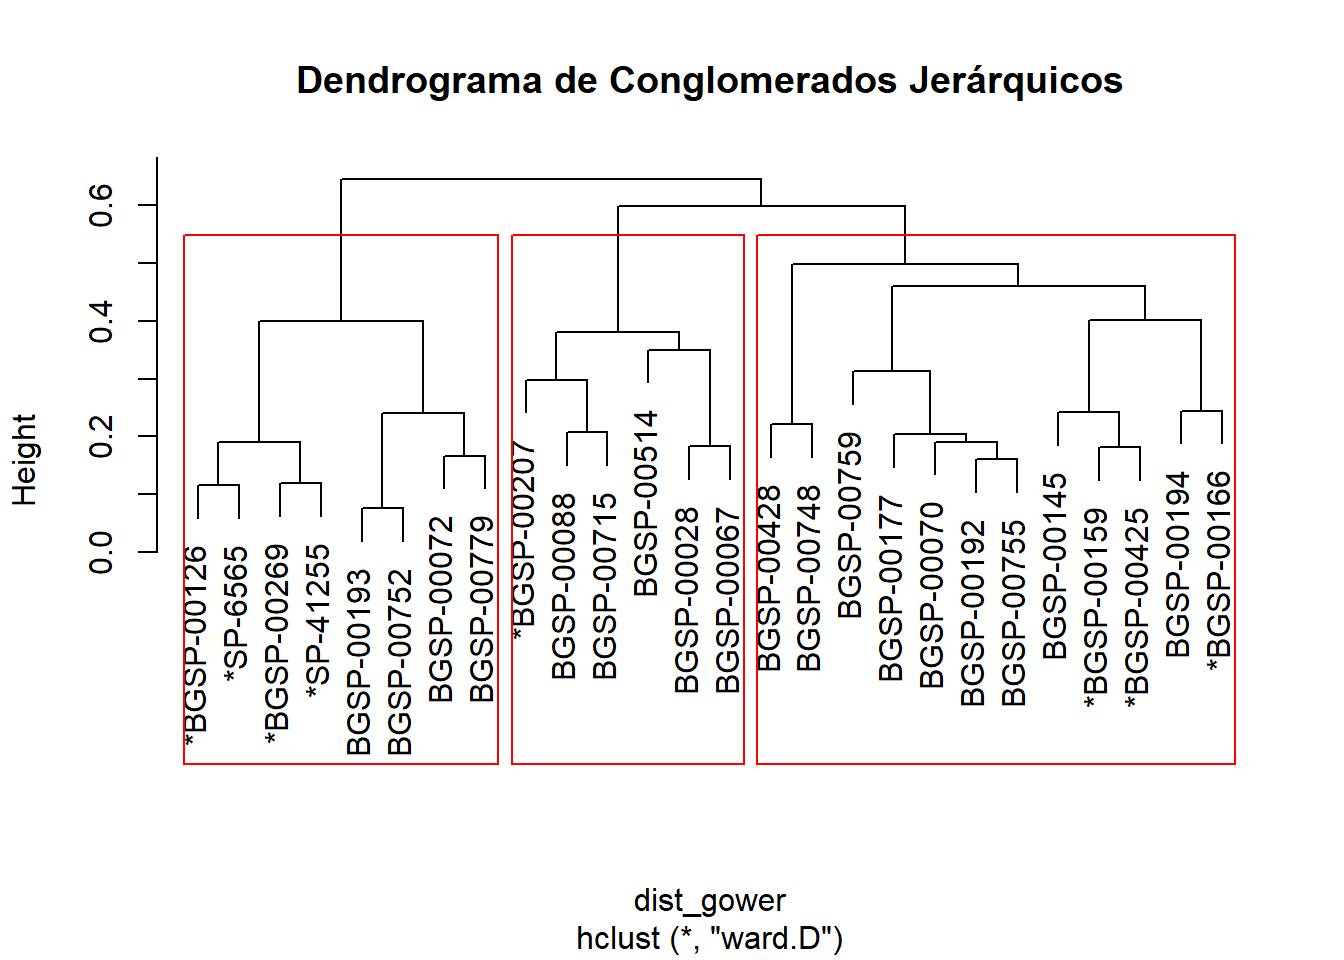
\includegraphics{Tesis_Dileo_files/figure-latex/cluster-1.pdf} 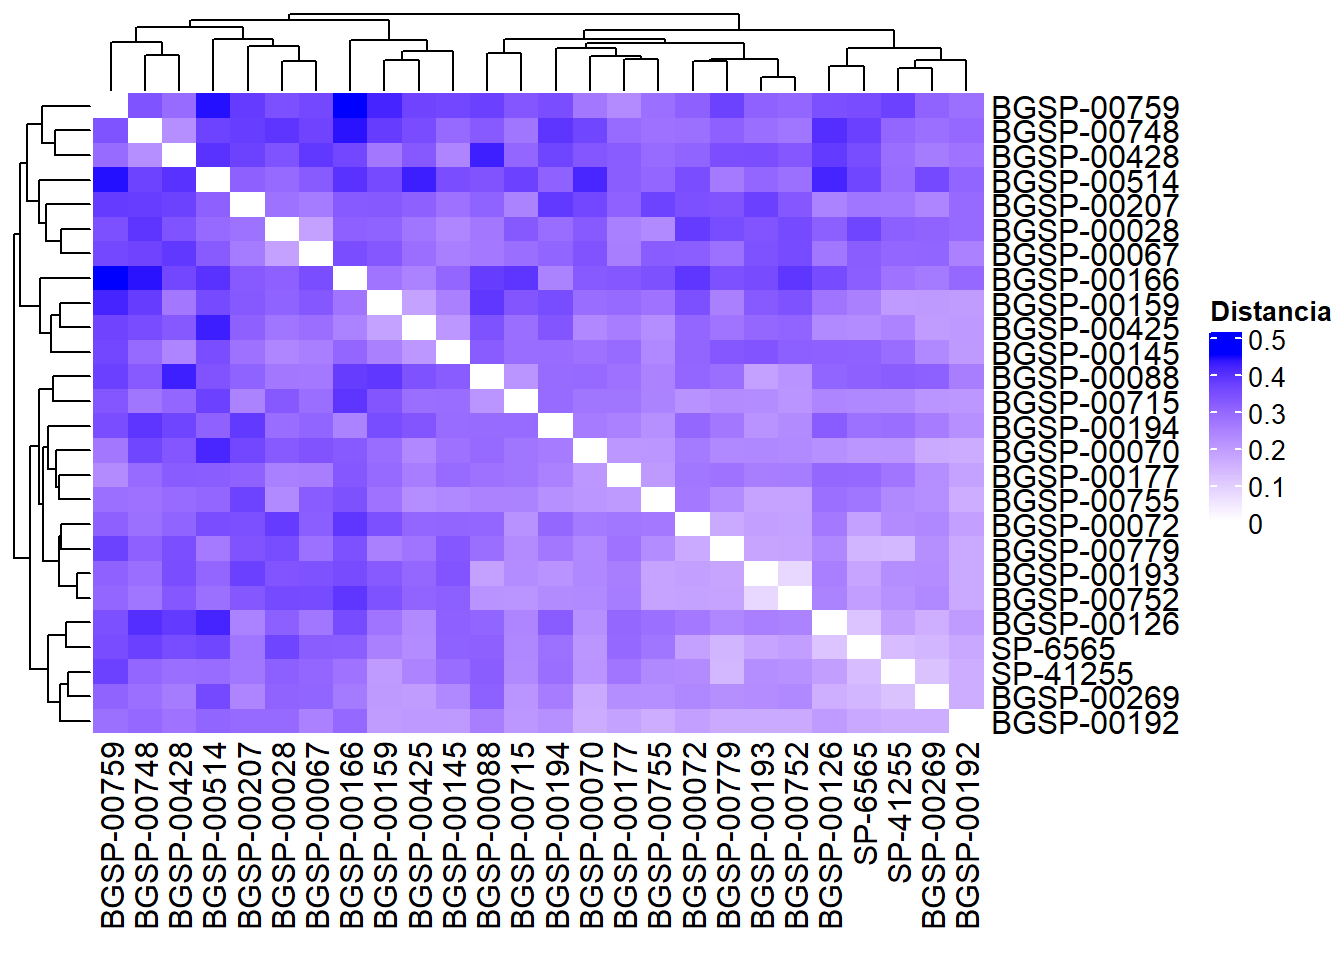
\includegraphics{Tesis_Dileo_files/figure-latex/cluster-2.pdf}

\subsection{\texorpdfstring{Caracterización de ocho entradas seleccionadas de algodón (\emph{Gossypium hirsutum} L.)}{Caracterización de ocho entradas seleccionadas de algodón (Gossypium hirsutum L.)}}\label{caracterizaciuxf3n-de-ocho-entradas-seleccionadas-de-algoduxf3n-gossypium-hirsutum-l.-1}

\subsubsection{Características de rendimiento y sus componentes y calidad de fibra}\label{caracteruxedsticas-de-rendimiento-y-sus-componentes-y-calidad-de-fibra}

Las entradas seleccionadas para una mayor profundización en la evaluación de las características de rendimiento y calidad se muestran en la tabla \ref{tab:table-charac}. La selección se realizó principalmente mediante los datos mostrados en la tabla \ref{tab:tabla-datos-conjuntos}, eligiendo entradas contrastantes en términos de rendimiento y sus componentes (principalmente RFD) y calidad de fibra. Adicionalmente, se seleccionaron algunas entradas que presentaban baja NRV y aspecto de canopia compacta, como es el caso de la entrada BGSP-00166.

\begin{table}[!h]
\centering\centering
\caption{\label{tab:table-charac}Valores medios, error estándar (entre paréntesis) y prueba L.S.D. (diferencia mínima significativa) de Fisher para rendimiento de fibra, sus componentes y calidad.}
\centering
\resizebox{\ifdim\width>\linewidth\linewidth\else\width\fi}{!}{
\fontsize{14}{16}\selectfont
\begin{threeparttable}
\begin{tabular}[t]{>{\raggedright\arraybackslash}p{2.5cm}>{\raggedright\arraybackslash}p{1cm}>{\raggedright\arraybackslash}p{1cm}>{\raggedright\arraybackslash}p{1cm}>{\raggedright\arraybackslash}p{1cm}>{\raggedright\arraybackslash}p{1cm}>{\raggedright\arraybackslash}p{1cm}>{\raggedright\arraybackslash}p{1cm}>{\raggedright\arraybackslash}p{1cm}>{\raggedright\arraybackslash}p{1cm}>{\raggedright\arraybackslash}p{1cm}>{\raggedright\arraybackslash}p{1cm}>{\raggedright\arraybackslash}p{1cm}}
\toprule
\multicolumn{1}{c}{ } & \multicolumn{8}{c}{Rendimiento y sus componentes} & \multicolumn{4}{c}{Calidad de fibra} \\
\cmidrule(l{3pt}r{3pt}){2-9} \cmidrule(l{3pt}r{3pt}){10-13}
\begingroup\fontsize{14}{16}\selectfont \textbf{Entradas}\endgroup & \begingroup\fontsize{14}{16}\selectfont \textbf{RB}\endgroup & \begingroup\fontsize{14}{16}\selectfont \textbf{RF}\endgroup & \begingroup\fontsize{14}{16}\selectfont \textbf{RFD}\endgroup & \begingroup\fontsize{14}{16}\selectfont \textbf{PC}\endgroup & \begingroup\fontsize{14}{16}\selectfont \textbf{NC}\endgroup & \begingroup\fontsize{14}{16}\selectfont \textbf{IS}\endgroup & \begingroup\fontsize{14}{16}\selectfont \textbf{IF}\endgroup & \begingroup\fontsize{14}{16}\selectfont \textbf{NSC}\endgroup & \begingroup\fontsize{14}{16}\selectfont \textbf{UHML}\endgroup & \begingroup\fontsize{14}{16}\selectfont \textbf{Str}\endgroup & \begingroup\fontsize{14}{16}\selectfont \textbf{Mic}\endgroup & \begingroup\fontsize{14}{16}\selectfont \textbf{IU}\endgroup\\
\midrule
 &  &  &  &  &  &  &  &  &  &  &  \vphantom{1} & \\
BGSP-00126 & 30,5 (6,6) & 13,2 (2,9) & 43,1 (0,4) & 3,6 (0,4) & 8,0 (1,0) & 8,7 (0,3) & 6,2 (0,3) & 25,0 (1,6) & 29,8 (0,3) & 30,4 (1,3) & 3,5 (0,4) & 83,8 (1,0)\\
BGSP-00159 & 26,2 (5,4) & 9,5 (1,9) & 36,3 (0,8) & 4,1 (0,5) & 6,2 (0,6) & 10,3 (1,0) & 5,6 (0,7) & 26,8 (0,7) & 28,4 (0,9) & 33,2 (2,1) & 3,7 (0,5) & 82,7 (0,5)\\
BGSP-00166 & 27,5 (4,3) & 8,6 (1,4) & 31,2 (0,3) & 4,6 (0,4) & 5,8 (0,5) & 11,5 (0,5) & 5,0 (0,4) & 28,9 (0,8) & 33,2 (0,5) & 37,3 (2,0) & 3,2 (0,3) & 85,8 (0,6)\\
BGSP-00207 & 30,2 (6,3) & 13,1 (2,7) & 43,5 (0,4) & 3,6 (0,4) & 8,0 (1,0) & 8,3 (0,2) & 6,2 (0,3) & 25,2 (2,0) & 28,3 (0,4) & 29,2 (0,7) & 3,4 (0,3) & 83,5 (0,4)\\
\addlinespace
BGSP-00269 & 29,8 (5,8) & 12,9 (2,5) & 43,4 (0,4) & 3,4 (0,2) & 8,6 (1,1) & 8,8 (0,4) & 6,5 (0,2) & 22,8 (1,9) & 28,3 (0,5) & 31,6 (1,2) & 4,3 (0,2) & 83,7 (0,3)\\
BGSP-00425 & 31,5 (7,4) & 11,3 (2,9) & 34,2 (1,2) & 3,6 (0,4) & 8,3 (1,1) & 7,9 (0,4) & 4,0 (0,6) & 30,6 (0,9) & 30,4 (1,0) & 31,3 (1,6) & 3,4 (0,5) & 82,2 (0,2)\\
SP-41255 & 34,2 (6,1) & 15,8 (3,0) & 45,8 (0,6) & 3,7 (0,5) & 9,2 (1,0) & 7,7 (0,1) & 6,2 (0,3) & 26,8 (2,8) & 29,8 (0,7) & 32,2 (1,2) & 3,8 (0,3) & 83,6 (0,7)\\
SP-6565 & 30,1 (5,8) & 12,5 (2,4) & 41,4 (1,0) & 3,7 (0,6) & 8,2 (0,7) & 8,9 (0,4) & 5,9 (0,2) & 25,5 (3,0) & 30,1 (0,5) & 32,5 (0,9) & 3,7 (0,3) & 84,9 (0,6)\\
 &  &  &  &  &  &  &  &  &  &  &  & \\
\addlinespace
p-value & 0,005 & <0,001 & <0,001 & 0,002 & <0,001 & <0,001 & <0,001 & 0,014 & <0,001 & 0,017 & <0,001 & 0,003\\
Fisher’s L.S.D & 3,68 & 1,91 & 1,99 & 0,57 & 1,19 & 1,35 & 0,75 & 4,04 & 1,38 & 4,03 & 0,43 & 1,66\\
\bottomrule
\end{tabular}
\begin{tablenotes}[para]
\item \textit{Referencias:} 
\item RB: Rendimiento de algodón bruto en g; RF: Rendimiento de fibra en g; RFD: Rendimiento de fibra al desmote en \%; PC: Peso promedio de capullos en g; NC: Número de capullos; IS: Índice de semillas en g; IF: Índice de fibra en g; NSC: Numero de semillas por capullo. UHML: Longitud promedio de fibra de la mitad superior en mm; Str: Resistencia de las fibras g tex\textsuperscript{-1}; Mic: Micronaire; IU: Índice de uniformidad de fibras en \%.
\end{tablenotes}
\end{threeparttable}}
\end{table}

Las entradas de algodón mostraron diferencias significativas en todos los rasgos relacionados con el rendimiento y la calidad de la fibra (p \textless{} 0,05, Tabla \ref{tab:table-charac}).

La entrada SP-41255 presentó los valores medios más elevados para RB, RF, RFD y NC, con valores de 34,2 g planta\textsuperscript{-1}, 15,8 g planta\textsuperscript{-1}, 45,8 \%, y 9,2 capullos planta\textsuperscript{-1} respectivamente, sin embargo, presentó el valor medio más bajo de IS, con 7,7 g. BGSP-00159 tuvo la media más baja de RB con 26,2 g planta\textsuperscript{-1}. BGSP-00166 tuvo los valores medios más bajos para RF, RFD, MIC y NC con valores de 8,6 g planta\textsuperscript{-1}, 31,1 \%, 3,2 y 5,8 capullos planta\textsuperscript{-1} respectivamente, no obstante, presentó los valores medios más elevados de PC, IS, UHML, Str y IU con valores de 4,6 g capullo\textsuperscript{-1}, 11,5 g, 33,2 mm, 37,3 g tex\textsuperscript{-1} y 85,8 \% respectivamente. BGSP-00269 presentó los valores medios más bajos de PC, NSC y UHML, con valores de 3,4 g capullo\textsuperscript{-1}, 22,8 semilla capullo\textsuperscript{-1}, y 28,3 mm respectivamente, mientras que tuvo el valor medio más alto para IF y Mic con valores de 6,5 g y 4,3. BGSP-00425 tuvo la NSC media mas alta, con un 30,6 semillas cápsula\textsuperscript{-1} mientras que los valores medios más bajos para IF y IU con valores de 4,0 g y 82,2 \%, respectivamente. BGSP-00207 presentó los valores medios más bajos de UHML y Str con valores de 28,3 mm y 29,2 g tex\textsuperscript{-1} respectivamente. En particular, las accesiones BGSP-00166 y SP-41255 fueron significativamente diferentes para casi todos los caracteres estudiados excepto para NSC (p \textless{} 0,01).

Estos resultados indican que existe variación fenotípica entre las accesiones de algodón tanto en términos de rendimiento como de calidad de la fibra.

En el analisis de componentes principales incluyendo todas las variables, el primer componente principal explicó el 45,6\% de la varianza de los datos, mientras que el segundo componente principal explicó el 21,9\% (Figura \ref{fig:img-PC}). Los rasgos más asociados con el primer componente fueron RB, Mic, RF, IF y NC, mientras que UHML, Str, IU, IS, NSC, PC y RFD fueron los más asociados con el segundo componente. Las entradas situadas en el cuadrante superior izquierdo fueron BGSP-00166, BGSP-00159 y BGSP-00425, estando estas entradas asociadas con valores más altos de calidad de fibra (UHML, Str, IU) y tamaño de semilla (IS) y valores más bajos en caracteres relacionados con el rendimiento como RB, RF, IF, NC, RFD. Las entradas situadas en el cuadrante inferior derecho como SP-41255, BGSP-00269, BGSP-00207 y BGSP-00126, mostraron un comportamiento opuesto a las descritas.

\begin{figure}
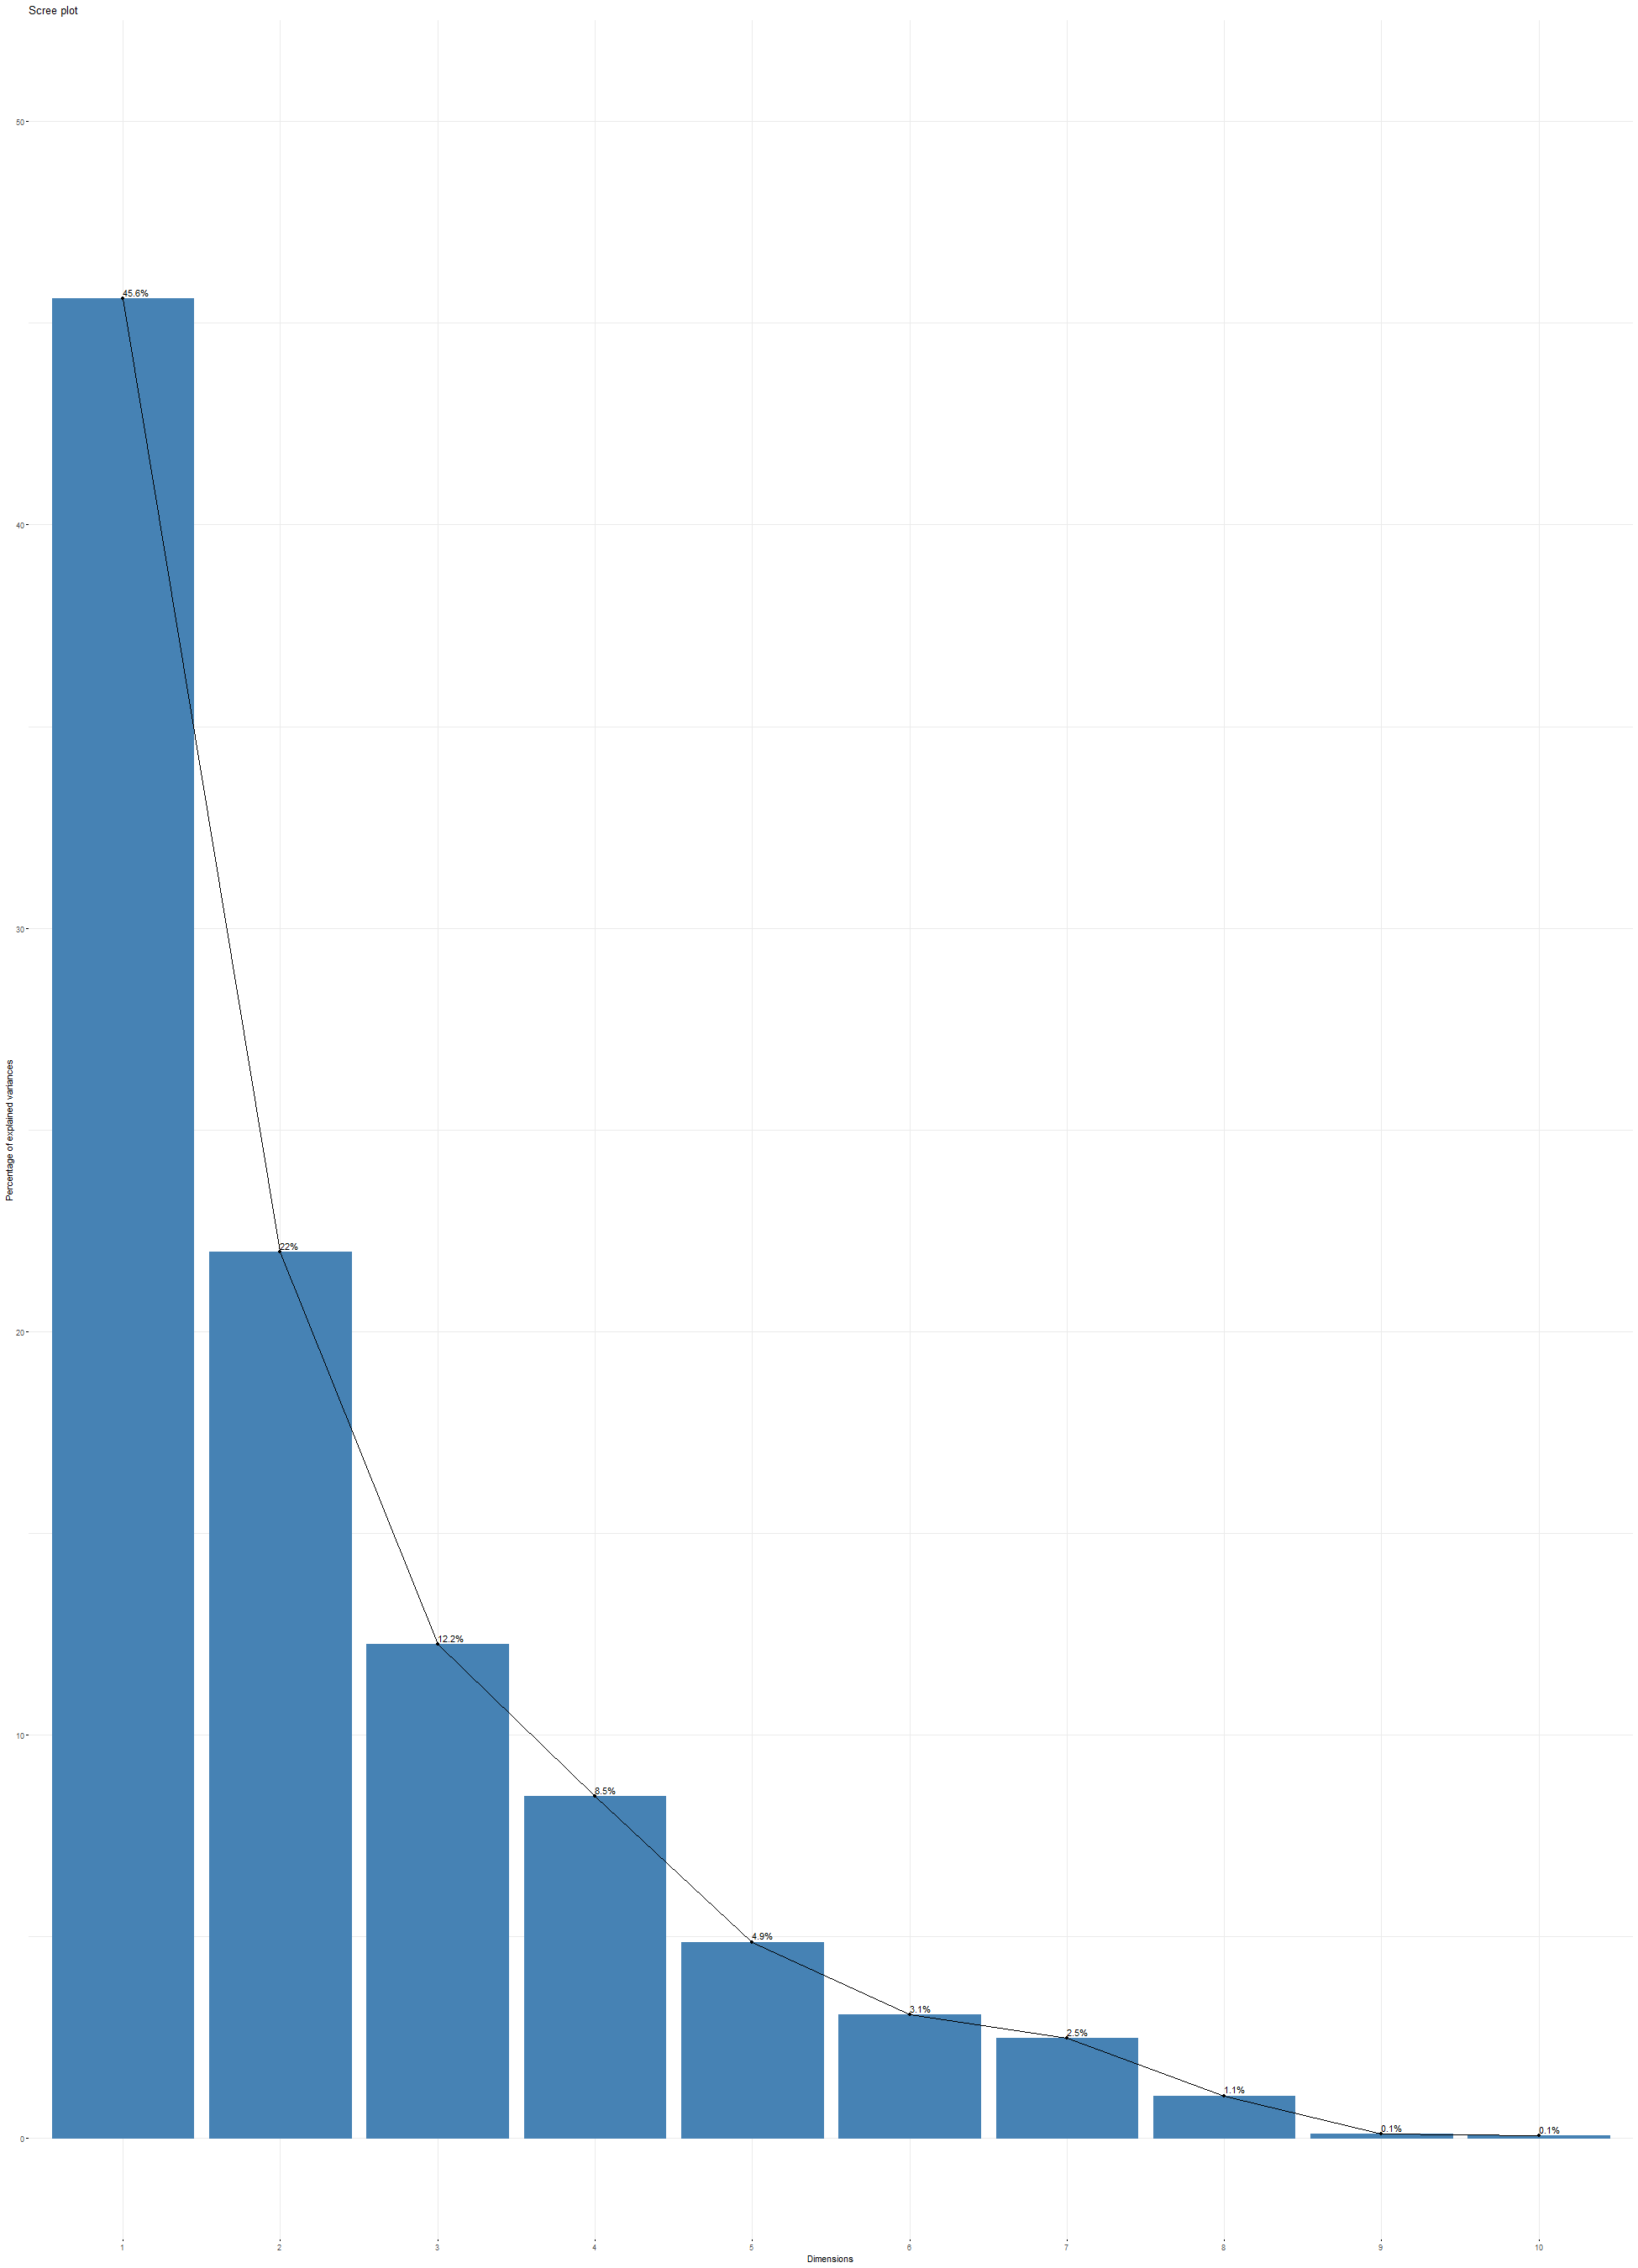
\includegraphics[width=400px]{figure/chap1/Para_compuestas/PCA_juntas} \caption{Biplot del análisis de componentes principales con puntos que representan las proyecciones de las accesiones (1) y las variables (2) en el espacio definido por las dos primeras dimensiones (Dim) o componentes principales. RB: Rendimiento de algodón bruto en g; RF: Rendimiento de fibra en g; RFD: Rendimiento de fibra al desmote en \%; PC: Peso promedio de capullos en g; NC: Número de capullos; IS: Índice de semillas en g; IF: Índice de fibra en g; NSC: Numero de semillas por capullo. UHML: Longitud promedio de fibra de la mitad superior en mm; Str: Resistencia de las fibras g tex\textsuperscript{-1}; Mic: Micronaire; IU: Índice de uniformidad de fibras en \%.}\label{fig:img-PC}
\end{figure}

En particular, las entradas BGSP-00166 y SP-41255 presentaron más contraste en cuanto a los rasgos medidos. Estas accesiones mostraron valores diferentes para la mayoría de los rasgos medidos relacionados tanto con el rendimiento como con la calidad de la fibra. Por lo tanto, seleccionamos estas accesiones para realizar un cruce biparental y generar una población segregante para estimar los parámetros genéticos y, a continuación, seleccionar fenotipos prometedores para el rendimiento y los rasgos relacionados con la calidad.

En la Tabla \ref{tab:correlation-greenhouse} se muestran los valores de correlación de Spearman para las caracteristicas de rendimiento de fibra, sus componentes y calidad de fibra.

\begin{table}[!h]
\centering
\caption{\label{tab:correlation-greenhouse}Correlación de Spearman entre los rasgos evaluados en el germoplasma de colección}
\centering
\resizebox{\ifdim\width>\linewidth\linewidth\else\width\fi}{!}{
\begin{threeparttable}
\begin{tabular}[t]{>{\raggedright\arraybackslash}p{3em}lllllllllll}
\toprule
  & RB & RF & RFD & PC & NC & IS & IF & NSC & UHML & Str & Mic\\
\midrule
RF & .94*** & - &  &  &  &  &  &  &  &  & \\
RFD & .24 & .48*** & - &  &  &  &  &  &  &  & \\
PC & .75*** & .67*** & -.15 & - &  &  &  &  &  &  & \\
NC & .86*** & .89*** & .42** & .43** & - &  &  &  &  &  & \\
IS & .01 & -.09 & -.51*** & .41** & -.27 & - &  &  &  &  & \\
\addlinespace
IF & .52*** & .70*** & .54*** & .49*** & .49*** & .20 & - &  &  &  & \\
NSC & .54*** & .38** & -.34* & .69*** & .30* & -.03 & -.06 & - &  &  & \\
UHML & -.35* & -.46** & -.36* & -.15 & -.42** & .14 & -.46** & .06 & - &  & \\
Str & -.14 & -.27 & -.42** & .07 & -.30* & .51*** & -.17 & -.08 & .38** & - & \\
Mic & .79*** & .83*** & .35* & .64*** & .77*** & .06 & .71*** & .28 & -.53*** & -.23 & -\\
\addlinespace
IU & -.05 & -.06 & -.01 & .09 & -.10 & .40** & .09 & -.14 & .34* & .46*** & -.10\\
\bottomrule
\end{tabular}
\begin{tablenotes}[para]
\item \textit{Referencias:} 
\item *p < 0.05, **p < 0.01 and *** p < 0.001. RB: Rendimiento de algodón bruto en g; RF: Rendimiento de fibra en g; RFD: Rendimiento de fibra al desmote en \%; PC: Peso promedio de capullos en g; NC: Número de capullos; IS: Índice de semillas en g; IF: Índice de fibra en g; NSC: Numero de semillas por capullo. UHML: Longitud promedio de fibra de la mitad superior en mm; Str: Resistencia de las fibras g tex\textsuperscript{-1}; Mic: Micronaire; IU: Índice de uniformidad de fibras en \%.
\end{tablenotes}
\end{threeparttable}}
\end{table}

Varias correlaciones fenotípicas fueron estadísticamente significativas (Tabla \ref{tab:correlation-greenhouse}). Para el análisis, se consideraron correlaciones fuertes los valores superiores a 0,80, moderadas las comprendidas entre 0,40 y 0,80, y bajas las inferiores a 0,40. El RF mostró una fuerte correlación positiva con el NC. También mostró una correlación positiva moderada con PC. La RFD mostró una correlación positiva moderada con el RF y el NC. Sin embargo, mostró una correlación negativa moderada con IS. El UHML mostró correlaciones negativas moderadas con el RF, lo que indica que, a medida que aumenta el rendimiento de fibra, disminuye la longitud de la misma.

\subsubsection{Procesos fisiológicos que intervienen en la determinación del rendimiento de fibra}\label{procesos-fisioluxf3gicos-que-intervienen-en-la-determinaciuxf3n-del-rendimiento-de-fibra}

Biomasa total y particionada

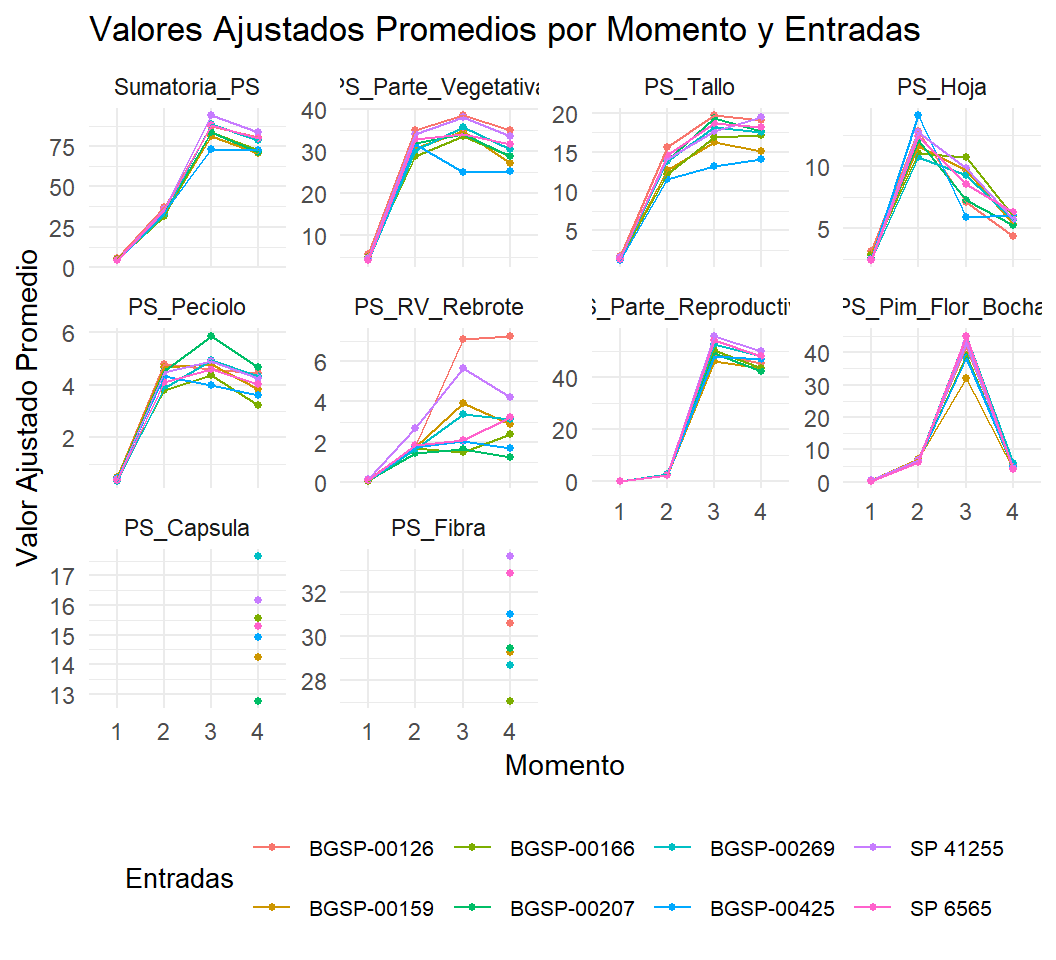
\includegraphics{Tesis_Dileo_files/figure-latex/Graficos-biomasa-1.pdf}

\begin{table}[!h]
\centering\centering
\caption{\label{tab:Anova-biomasa-particion-rep2}Acumulacion de biomasa en estructuras vegetativas, tallo, hojas, peciolos, ramas vegetativas, rebrote, biomasa reproductiva, pimpollo, flor, bocha, cápsula, semilla}
\centering
\resizebox{\ifdim\width>\linewidth\linewidth\else\width\fi}{!}{
\fontsize{12}{14}\selectfont
\begin{tabular}[t]{llrrrl}
\toprule
\multicolumn{1}{c}{ } & \multicolumn{5}{c}{ANOVA} \\
\cmidrule(l{3pt}r{3pt}){2-6}
\begingroup\fontsize{12}{14}\selectfont \textbf{Rasgos}\endgroup & \begingroup\fontsize{12}{14}\selectfont \textbf{Fuente}\endgroup & \begingroup\fontsize{12}{14}\selectfont \textbf{GLNum}\endgroup & \begingroup\fontsize{12}{14}\selectfont \textbf{GLDen}\endgroup & \begingroup\fontsize{12}{14}\selectfont \textbf{F}\endgroup & \begingroup\fontsize{12}{14}\selectfont \textbf{p-valor}\endgroup\\
\midrule
Biomasa Total & (Intercept) & 1 & 193 & 62.54 & <0.0001\\
 & Momento & 3 & 21 & 92.71 & <0.0001\\
 & Entradas & 7 & 193 & 6.34 & <0.0001\\
 & Momento:Entradas & 21 & 193 & 2.37 & 0.0011\\
1 Biomasa Vegetativa & (Intercept) & 1 & 193 & 210.27 & <0.0001\\
\addlinespace
 & Momento & 3 & 21 & 196.04 & <0.0001\\
 & Entradas & 7 & 193 & 4.55 & 0.0001\\
 & Momento:Entradas & 21 & 193 & 1.65 & 0.0416\\
1.1 Tallo & (Intercept) & 1 & 193 & 332.03 & <0.0001\\
 & Momento & 3 & 21 & 249.72 & <0.0001\\
\addlinespace
 & Entradas & 7 & 193 & 6.30 & <0.0001\\
 & Momento:Entradas & 21 & 193 & 2.41 & 0.0009\\
1.2 Hoja & (Intercept) & 1 & 193 & 211.00 & <0.0001\\
 & Momento & 3 & 21 & 39.10 & <0.0001\\
 & Entradas & 7 & 193 & 0.70 & 0.6741\\
\addlinespace
 & Momento:Entradas & 21 & 193 & 1.81 & 0.0195\\
1.3 Peciolo+Ramas & (Intercept) & 1 & 193 & 148.48 & <0.0001\\
 & Momento & 3 & 21 & 123.02 & <0.0001\\
 & Entradas & 7 & 193 & 2.73 & 0.0102\\
 & Momento:Entradas & 21 & 193 & 1.46 & 0.0956\\
\addlinespace
1.4 RV+Rebrote & (Intercept) & 1 & 193 & 63.81 & <0.0001\\
 & Momento & 3 & 21 & 21.61 & <0.0001\\
 & Entradas & 7 & 193 & 4.02 & 0.0004\\
 & Momento:Entradas & 21 & 193 & 1.49 & 0.0829\\
2 Biomasa Reproductiva & (Intercept) & 1 & 193 & 10.52 & 0.0014\\
\addlinespace
 & Momento & 3 & 21 & 62.70 & <0.0001\\
 & Entradas & 7 & 193 & 3.15 & 0.0035\\
 & Momento:Entradas & 21 & 193 & 1.45 & 0.0992\\
2.1 Prim+Flor+Bocha & (Intercept) & 1 & 193 & 132.53 & <0.0001\\
 & Momento & 3 & 21 & 94.71 & <0.0001\\
\addlinespace
 & Entradas & 7 & 193 & 0.94 & 0.4797\\
 & Momento:Entradas & 21 & 193 & 0.63 & 0.8961\\
2.2 Cápsula (M4) & (Intercept) & 1 & 47 & 10.82 & 0.0019\\
 & Entradas & 7 & 47 & 3.85 & 0.0022\\
2.3 Fibra+Semilla (M4) & (Intercept) & 1 & 47 & 13.01 & 0.0007\\
\addlinespace
 & Entradas & 7 & 47 & 2.36 & 0.0373\\
\bottomrule
\end{tabular}}
\end{table}

Retención global

\begin{table}[!h]
\centering\centering
\caption{\label{tab:Anova-retencion}Retención global, y en posiciones 1, 2 y 3, en los momentos M2, M3, y M4}
\centering
\resizebox{\ifdim\width>\linewidth\linewidth\else\width\fi}{!}{
\fontsize{12}{14}\selectfont
\begin{tabular}[t]{llrrrl}
\toprule
\multicolumn{1}{c}{ } & \multicolumn{5}{c}{ANOVA} \\
\cmidrule(l{3pt}r{3pt}){2-6}
\begingroup\fontsize{12}{14}\selectfont \textbf{Rasgos}\endgroup & \begingroup\fontsize{12}{14}\selectfont \textbf{Fuente}\endgroup & \begingroup\fontsize{12}{14}\selectfont \textbf{GLNum}\endgroup & \begingroup\fontsize{12}{14}\selectfont \textbf{GLDen}\endgroup & \begingroup\fontsize{12}{14}\selectfont \textbf{F}\endgroup & \begingroup\fontsize{12}{14}\selectfont \textbf{p-valor}\endgroup\\
\midrule
Ret\_Global & (Intercept) & 1 & 144 & 90.21 & <0.0001\\
 & Momento & 2 & 14 & 52.91 & <0.0001\\
 & Entradas & 7 & 144 & 3.48 & 0.0018\\
 & Momento:Entradas & 14 & 144 & 2.21 & 0.0098\\
Ret\_P1 & (Intercept) & 1 & 144 & 338.14 & <0.0001\\
\addlinespace
 & Momento & 2 & 14 & 89.26 & <0.0001\\
 & Entradas & 7 & 144 & 1.47 & 0.1810\\
 & Momento:Entradas & 14 & 144 & 3.05 & 0.0004\\
Ret\_P2 & (Intercept) & 1 & 144 & 22.78 & <0.0001\\
 & Momento & 2 & 14 & 8.89 & 0.0032\\
\addlinespace
 & Entradas & 7 & 144 & 2.65 & 0.0131\\
 & Momento:Entradas & 14 & 144 & 1.29 & 0.2206\\
Ret\_P3 & (Intercept) & 1 & 144 & 13.92 & 0.0003\\
 & Momento & 2 & 14 & 6.59 & 0.0096\\
 & Entradas & 7 & 144 & 1.06 & 0.3914\\
\addlinespace
 & Momento:Entradas & 14 & 144 & 0.92 & 0.5359\\
\bottomrule
\end{tabular}}
\end{table}

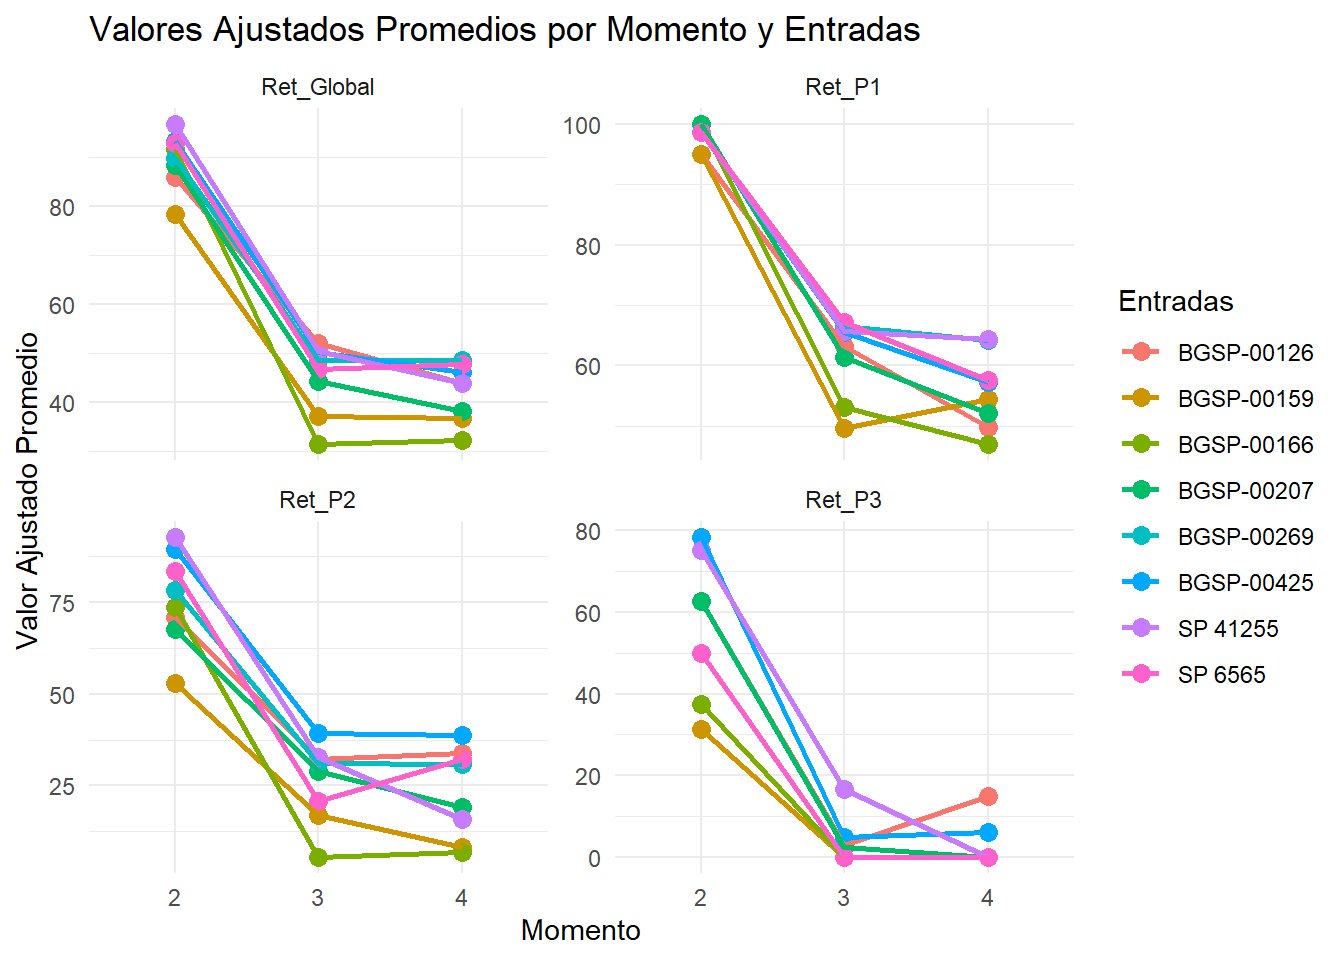
\includegraphics{Tesis_Dileo_files/figure-latex/Anova-retencion-1.pdf}

Fotosíntesis, conductancia estomática y SPAD

\begin{table}[!h]
\centering\centering
\caption{\label{tab:Anova-fotosintesis-cond-spad}Fotosintesis, conductancia estomatica y SPAD}
\centering
\resizebox{\ifdim\width>\linewidth\linewidth\else\width\fi}{!}{
\fontsize{12}{14}\selectfont
\begin{tabular}[t]{llrrrl}
\toprule
\multicolumn{1}{c}{ } & \multicolumn{5}{c}{ANOVA} \\
\cmidrule(l{3pt}r{3pt}){2-6}
\begingroup\fontsize{12}{14}\selectfont \textbf{Rasgos}\endgroup & \begingroup\fontsize{12}{14}\selectfont \textbf{Fuente}\endgroup & \begingroup\fontsize{12}{14}\selectfont \textbf{GLNum}\endgroup & \begingroup\fontsize{12}{14}\selectfont \textbf{GLDen}\endgroup & \begingroup\fontsize{12}{14}\selectfont \textbf{F}\endgroup & \begingroup\fontsize{12}{14}\selectfont \textbf{p-valor}\endgroup\\
\midrule
SPAD & (Intercept) & 1 & 56 & 139.88 & <0.0001\\
 & DDE & 1 & 56 & 19.76 & <0.0001\\
 & Entradas & 7 & 21 & 1.04 & 0.4363\\
 & DDE:Entradas & 7 & 56 & 0.74 & 0.6355\\
Cond & (Intercept) & 1 & 56 & 26.32 & <0.0001\\
\addlinespace
 & DDE & 1 & 56 & 1.18 & 0.2814\\
 & Entradas & 7 & 21 & 0.90 & 0.5224\\
 & DDE:Entradas & 7 & 56 & 0.91 & 0.5085\\
Photo & (Intercept) & 1 & 56 & 339.17 & <0.0001\\
 & DDE & 1 & 56 & 122.17 & <0.0001\\
\addlinespace
 & Entradas & 7 & 21 & 3.49 & 0.0122\\
 & DDE:Entradas & 7 & 56 & 3.36 & 0.0046\\
\bottomrule
\end{tabular}}
\end{table}

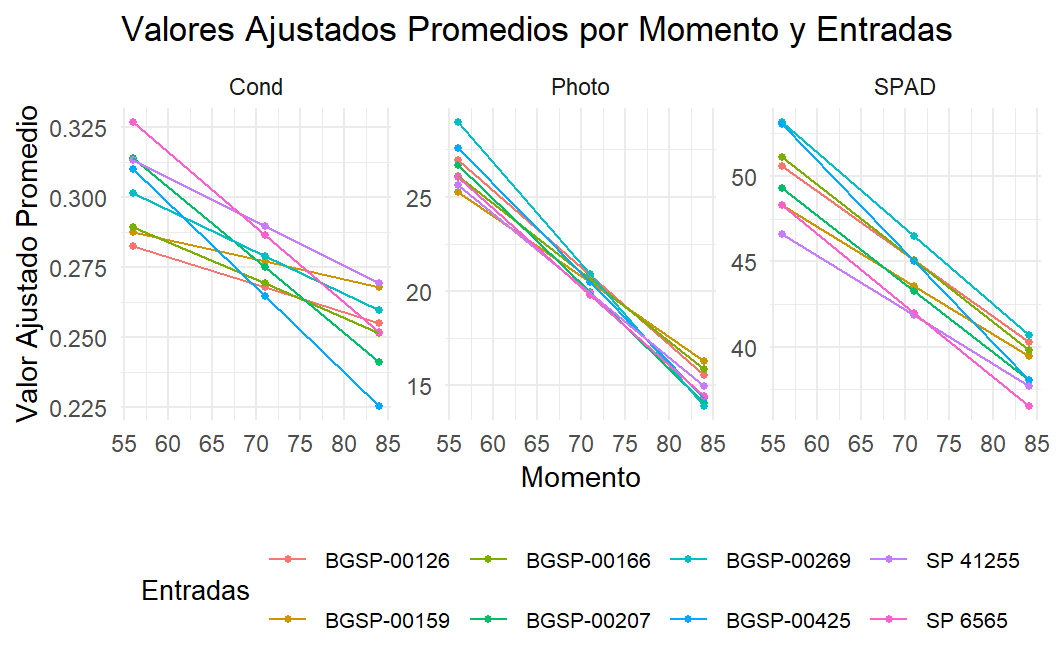
\includegraphics{Tesis_Dileo_files/figure-latex/Anova-fotosintesis-cond-spad-1.pdf}

\section{Discusión}\label{discusiuxf3n}

Aquí la discusión del capítulo 1

plant mapping specifically refers to the recording and evaluating of plant structure and the distribution and retention of fruit on plants at a specific time \autocite{kerby2010}

\section{Conclusión}\label{conclusiuxf3n}

Aquí la conclusión del capítulo 1

\chapter{Identificación de QTL de importancia agronómica}\label{math-sci}

\section{Introducción}\label{introducciuxf3n-2}

Aquí una breve introducción del capítulo

\section{Objetivo}\label{objetivo}

Mapear QTL (Quantitative Trait Loci) asociados a caracteres de rendimiento de fibra mediante el análisis de una población segregante F\textsubscript{2} obtenida del cruzamiento de progenitores contrastantes.

\section{Materiales y métodos}\label{materiales-y-muxe9todos-1}

Se caracterizaron marcadores moleculares del tipo SSR (Single Sequence Repeats o microsatélites) asociados a QTLs de importancia agronómica. Se utilizaron 55 SSR \textbf{\texttt{chequear\ n°\ de\ marcadores}} que fueron seleccionados acorde tanto a trabajos científicos \autocite{zhang2005,shen2007,wang2007,wang2014,xia2014,wang2015,an2010,liu2012,qin2015,shi2015,su2016,zhang2016,ademe2017,liu2017,iqbal2017,li2017,baytar2018,liu2018} como la base de datos de CottonGen (\url{http://www.cottongen.org}). Dicha actividad se realizó en el laboratorio de biotecnología de INTA Reconquista. A partir de las entradas contrastantes para las características de interés, se realizaron cruzamientos y por autofecundación de las F\textsubscript{1} se obtuvo la población F\textsubscript{2}. A continuación, se detallan las etapas:

\begin{enumerate}
\def\labelenumi{\roman{enumi}.}
\item
  Obtención de la poblacion segregante para los loci de los marcadores (M) y los QTLs. Luego de la caracterización morfológica y fisiológica, las entradas fueron seleccionadas para ser utilizadas como parentales contrastantes en los respectivos cruzamientos de este estudio. Para los mismos se utilizaron las entradas de alto porcentaje de desmote como parentales masculinos. Considerando que por cada bocha se obtiene, en promedio, 20 semillas \autocite{naeem2017} se tomó una flor de cada parental para dicho cruzamiento, para la generación de la población F\textsubscript{1} (20 plantas). La población segregante (F\textsubscript{2}) resultó de la autofecundación de las F\textsubscript{1}, para llegar a una población F\textsubscript{2} aproximada de 200 plantas \autocite{bardak2018,zhang2003}.

  BGSP-00166 y SP-41255 fueron los genotipos parentales seleccionados. Ambos parentales son de origen argentino. El primer parental es una línea endogámica derivada del cruce entre Chaco 510 x SP 6269, mientras que el segundo parental es otra línea endogámica seleccionada del cruce entre SP-81270-7 x Mij. 3.Morfológicamente, difieren en su estructura de planta (Figure \ref{fig:img-parental}). BGSP-00166 es más compacta, con una distancia más corta entre la primera posición de fructificación y el tallo, mientras que SP-41255 tiene una estructura de planta más abierta. El cruzamiento se realizó en ambas direcciones para evaluar la existencia de efecto recíproco. La emasculación se realizó en las plantas utilizadas como parentales femeninos mediante la eliminación de los estambres con pinzas antes de la antesis floral (estadio en forma de vela), durante las horas de la tarde. Al día siguiente, se realizó el cruce mediante la transferencia de polen de los parentales masculinos a los femeninos (flores emasculadas), tal y como se describe en \textcite{acquaah2012}. A continuación, las semillas F\textsubscript{1} de los cruces de algodón se sembraron en condiciones de invernadero y se autopolinizaron para producir F\textsubscript{2}. En la temporada de cultivo 2019-2020, la población F\textsubscript{2} se sembró en hileras no replicadas en condiciones de campo. Cada hilera tenía 10 m de longitud y una separación de 1 m, con 50 plantas por hilera (Figura \ref{fig:img-croquis}). Las generaciones no segregantes (tanto las F\textsubscript{1}s, SP-41255 x BGSP-00166 y BGSP-00166 x SP-41255, como los genotipos parentales) también se sembraron en las mismas condiciones. Todas estas generaciones se sometieron a evaluación fenotípica. En la dirección de cruzamiento de SP-41255 x BGSP-00166, se consiguió una población segregante F\textsubscript{2} de 205 plantas, mientras que para la dirección de cruzamiento inversa, se obtuvieron 234 plantas. En el mismo ensayo, como se muestra en la Figura \ref{fig:img-croquis}, se sembraron y consiguieron uniformemente 17 plantas del progenitor BGSP-00166, 19 plantas del progenitor SP-41255 y 11 plantas de la F\textsubscript{1} (mitad y mitad generadas a partir de una dirección de cruzamiento y su recíproca).
\item
  Medición de la característica fenotípica controlada por los QTL. Se realizarán las mediciones de rendimiento y calidad de fibra detalladas en el apartado ¨Caracterización morfológica¨. Para el experimento del cruce biparental, cada planta (de poblaciones segregantes y no segregantes) también se cosechó individualmente en la fase de madurez para evaluar el rendimiento y las características relacionadas con la calidad: SCY, LY, LP, BW, BN, FL, FS, FU y MIC se midieron como se ha descrito anteriormente.
\item
  Caracterización molecular por SSR de los de los parentales y cada planta de la población F\textsubscript{2}. El ADN genómico se aisló utilizando hojas jóvenes procedentes de los progenitores y la población segregante, mediante método CTAB modificado \autocite{zhang2000,paterson1993}. Se evaluó la cantidad y calidad del ADN mediante espectrofotometría para comparación. La amplificación por PCR y la tinción con plata se realizó según \textcite{lin2005} . Los productos de PCR de los SSR se separaron en geles de poliacrilamida desnaturalizantes al \texttt{2\%} y revelados con carbonato de sodio\autocite{lin2005}.
\end{enumerate}

\begin{figure}
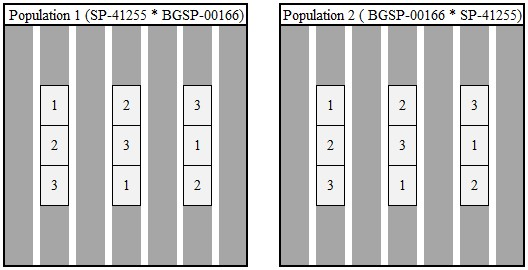
\includegraphics[width=400px]{figure/chap3/croquis_campo} \caption{Descripción del ensayo de campo, mostrando las dos poblaciones generadas a partir del cruce en la dirección SP-41255 x BGSP-00166 y su recíproco. En el ensayo se distribuyeron al azar plantas del parental SP-41255 (1), Filial 1 (2) y del parental BGSP-00166 (3).}\label{fig:img-croquis}
\end{figure}

\subsection{Análisis estadístico}\label{anuxe1lisis-estaduxedstico-1}

Para el experimento de cruzamiento biparental, se realizó una prueba de Levene para confirmar la varianza homogénea en las generaciones no segregantes, mientras que la distribución normal se confirmó mediante la prueba de Shapiro-Wilk. Se realizó la prueba L.S.D. de Fisher para comparar las parentales P\textsubscript{1}, P\textsubscript{2} y la generación F\textsubscript{1}. Además, también se realizó una comparación de las medias de las generaciones F\textsubscript{1} y F\textsubscript{2} recíprocas para detectar la existencia de un efecto recíproco en las características objeto de estudio. Se realizó un test de bondad de ajuste Chi-Cuadrado para detectar segregación transgresiva siguiendo el enfoque propuesto por \textcite{rodriguez2005} . Se consideró que la generación parental tenía un tamaño igual al de la generación F\textsubscript{2}. Las frecuencias esperadas se calcularon asumiendo igual tamaño entre la generación parental y la F\textsubscript{2}, y se consideraron fenotipos extremos aquellos individuos de la F\textsubscript{2} que superaban la media del rasgo en la generación parental y dos desvíos estándar (test de una cola, el 2,5\% de los individuos en una distribución normal). Bajo estos supuestos, cuando la proporción observada de individuos extremos en la generación F\textsubscript{2} superaba esta proporción esperada (un χ\textsuperscript{2} significativo), se consideraba que el rasgo mostraba un patrón de herencia transgresivo.

La heredabilidad en sentido amplio (\(h_{bs}^{2}\)) se estimó a partir de los componentes de varianza de las generaciones no segregantes (P\textsubscript{1}, P\textsubscript{2} and F\textsubscript{1}) y de la generación F2 de la siguiente manera \autocite{kearsey1996}:

\[ h_{bs}^{2}=\frac{\sigma^{^2}G}{\sigma^{2}Ph}\times100 \]

Donde \(h_{bs}^{2}\)= heredabilidad en sentido amplio, \(\sigma^{2}G\) = varianza genotípica, \(\sigma^{2}Ph\) = varianza fenotípica.

La varianza entre plantas dentro de las F\textsubscript{1}´s y los parentales P\textsubscript{1} y P\textsubscript{2} se consideró como varianza ambiental y se restó de la varianza entre plantas F\textsubscript{2} para obtener estimaciones de la varianza genotípica.

\[ \sigma^{2} E = \frac{\sigma^{2}P_1 + \sigma^{2}P_2 + \sigma^{2}F_1}{3} \]

Donde \(\sigma^{2}E\) = Varianza ambiental, \(\sigma^{2}P_1\) = Varianza del parental 1, \(\sigma^{2}P_2\) = Varianza del parental 2, \(\sigma^{2}F_1\) = varianza de la generación F\textsubscript{1} .

\[ \sigma^{2}G = \sigma^{2}Ph - \sigma^{2}E \]

Para estimar la correlación genética entre rasgos se utilizó la metodología propuesta por \textcite{kearsey1996} .

\section{Resultados}\label{resultados-1}

\begin{figure}
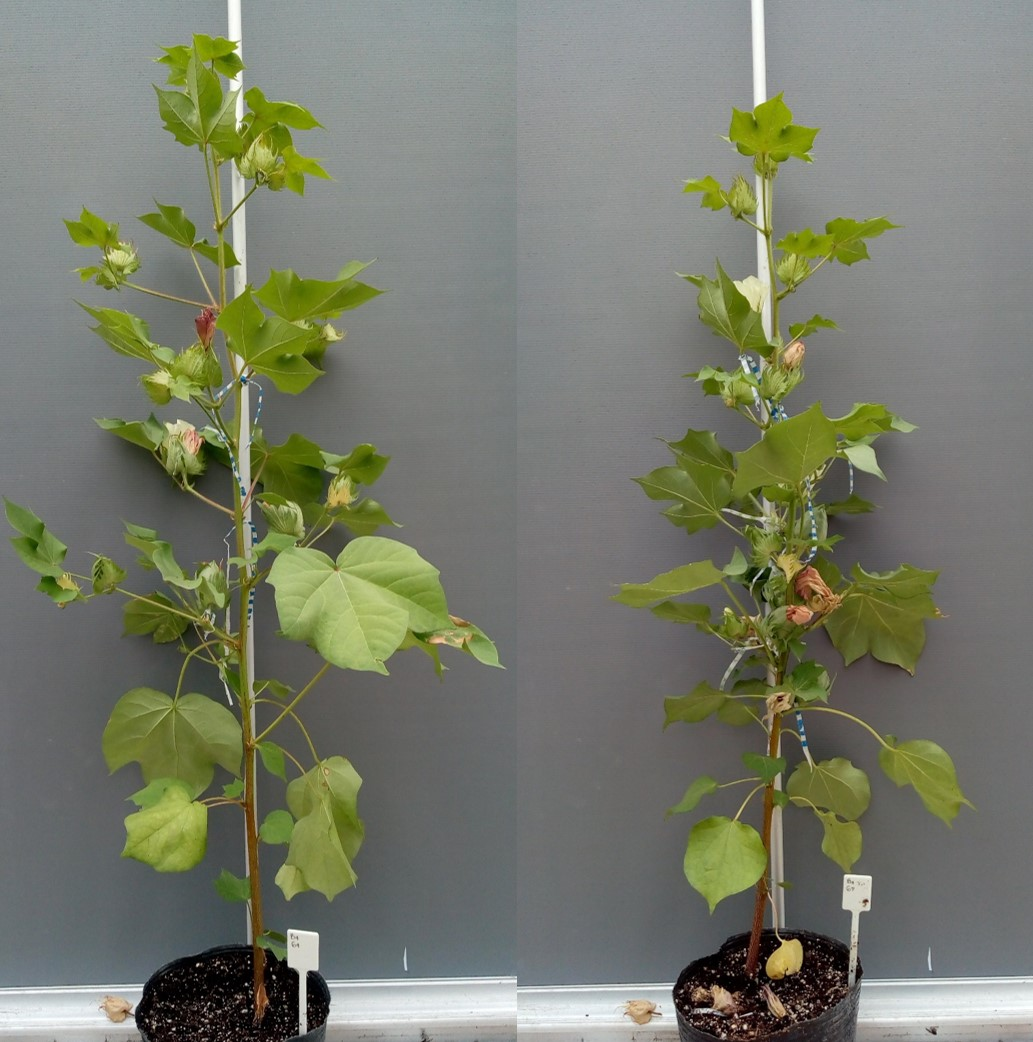
\includegraphics[width=400px]{figure/chap3/Parentales} \caption{Planta de los genotipos parentales SP-41255 y BGSP-00166}\label{fig:img-parental}
\end{figure}

\subsection{Generación de variabilidad a partir del cruce biparental BGSP-00166 x SP-41255}\label{generaciuxf3n-de-variabilidad-a-partir-del-cruce-biparental-bgsp-00166-x-sp-41255}

Los genotipos parentales BGSP-00166 y SP-41255 fueron significativamente diferentes para todos los caracteres evaluados, a excepción de RB(Tabla \ref{tab:table-generations-two}). Por otra parte, los valores medios de todos los caracteres no mostraron diferencias significativas entre la F\textsubscript{1} y la F\textsubscript{2} recíproca (p \textgreater{} 0,05), como se muestra en la Tabla S1. Esto significa que no existe el efecto recíproco en este cruce para los caracteres analizados. Por lo tanto, decidimos fusionar las poblaciones recíprocas F\textsubscript{1} y F\textsubscript{2}.

\begin{table}[!h]
\centering\centering
\caption{\label{tab:table-generations-two}Mean and variance (in parentheses) of the traits in the non-segregating generations (BGSP-00166, SP-41255 and F1) and the segregating generation F2}
\centering
\resizebox{\ifdim\width>\linewidth\linewidth\else\width\fi}{!}{
\fontsize{14}{16}\selectfont
\begin{tabular}[t]{>{\raggedright\arraybackslash}p{2.5cm}>{\raggedright\arraybackslash}p{1cm}>{\raggedright\arraybackslash}p{1cm}>{\raggedright\arraybackslash}p{1cm}>{\raggedright\arraybackslash}p{1cm}>{\raggedright\arraybackslash}p{1cm}>{\raggedright\arraybackslash}p{1cm}>{\raggedright\arraybackslash}p{1cm}>{\raggedright\arraybackslash}p{1cm}>{\raggedright\arraybackslash}p{1cm}>{}p{1cm}>{}p{1cm}>{}p{1cm}}
\toprule
\multicolumn{1}{c}{ } & \multicolumn{9}{c}{Caracteres} \\
\cmidrule(l{3pt}r{3pt}){2-10}
\begingroup\fontsize{14}{16}\selectfont \textbf{Generations}\endgroup & \begingroup\fontsize{14}{16}\selectfont \textbf{SCY}\endgroup & \begingroup\fontsize{14}{16}\selectfont \textbf{LY}\endgroup & \begingroup\fontsize{14}{16}\selectfont \textbf{LP}\endgroup & \begingroup\fontsize{14}{16}\selectfont \textbf{BW}\endgroup & \begingroup\fontsize{14}{16}\selectfont \textbf{BN}\endgroup & \begingroup\fontsize{14}{16}\selectfont \textbf{FL}\endgroup & \begingroup\fontsize{14}{16}\selectfont \textbf{FS}\endgroup & \begingroup\fontsize{14}{16}\selectfont \textbf{MIC}\endgroup & \begingroup\fontsize{14}{16}\selectfont \textbf{FU}\endgroup\\
\midrule
BGSP-00166 & 89.5a (1266.4) & 25.8a (110.3) & 30.9a (0.9) & 6.2b (0.4) & 14.5a (29.8) & 32.5b (0.3) & 37.1b (2.8) & 3.9a (0.1) & 85.5b (1.8)\\
SP-41255 & 86.9a (761.8) & 36.6b (126.1) & 43.4c (0.8) & 4.6a (0.3) & 19.1b (29.6) & 26.9a (0.6) & 30.7a (2.9) & 4.8c (0.1) & 82.0a (2.1)\\
F\textasciitilde{}1\textasciitilde{} & 123.5b (1013.1) & 44.1b (126.6) & 37.4b (0.4) & 6.4b (0.6) & 19.4b (26.7) & 32.0b (0.3) & 37.4b (0.9) & 4.2b (0.1) & 86.1b (0.9)\\
F\textasciitilde{}2\textasciitilde{} & 114.1 (1957.2) & 37.5 (227.3) & 37.2 (4.4) & 5.9 (0.9) & 19.7 (52.5) & 31.3 (1.5) & 36.1 (5.2) & 4.3 (0.2) & 84.9 (1.7)\\
\bottomrule
\multicolumn{10}{l}{\textsuperscript{} \makecell[l]{RB: Seed cotton yield in g, LY: Lint yield in g, \\ LP: Lint percentage in \%, BW: Boll weight in g, BN: Boll number \\ per plant, SI: Seed index in g, LI: Lint index in g, SNPB: Seed \\ number per boll, FL: Fibre length in mm, FS: Fibre strength \\ g tex\textasciicircum{}-1\textasciicircum{}, Mic: Micronaire, FU: Fibre uniformity in \%.}}\\
\end{tabular}}
\end{table}

\section{Discusión}\label{discusiuxf3n-1}

Aquí la discusión del capítulo 3

\section{Conclusión}\label{conclusiuxf3n-1}

Aquí la conclusión del capítulo 3\\

\hfill\break

\chapter{Si es necesario un tercer capítulo}\label{ref-labels}

\section{Introducción}\label{introducciuxf3n-3}

Aquí una breve introducción del capítulo

\section{Objetivo}\label{objetivo-1}

Aquí objetivo del capítulo 3

\section{Materiales y métodos}\label{materiales-y-muxe9todos-2}

Aquí M y M del capítulo 3

\section{Discusión}\label{discusiuxf3n-2}

Aquí la discusión del capítulo 3

\section{Conclusión}\label{conclusiuxf3n-2}

Aquí la conclusión del capítulo 3\\

\hfill\break

\chapter*{Conclusión}\label{conclusiuxf3n-3}
\addcontentsline{toc}{chapter}{Conclusión}

Las conclusiones de la tesis aquí..

\appendix

\chapter{Primer Apéndice}\label{primer-apuxe9ndice}

Sí es necesario incluir un apéndice, iría aquí..

\textbf{En capítulo \ref{rmd-basics}:}

Descripción aquí..

\chapter{Segundo Apéndice}\label{segundo-apuxe9ndice}

Este sería el segundo apéndice..

\backmatter

\chapter*{Referencias}\label{referencias}
\addcontentsline{toc}{chapter}{Referencias}

\printbibliography[heading=none]

\markboth{Referencias}{Referencias}

\noindent

\setlength{\parindent}{-0.20in}


% Index?

\end{document}
